\documentclass[12pt,letterpaper]{report}

% Preamble for co456_notes.tex

\usepackage[dvipsnames, table]{xcolor}

\usepackage{amsmath}
\usepackage{amssymb}
\usepackage{amsthm}
\usepackage{changepage}
\usepackage{enumitem}
\usepackage{fancyhdr}
\usepackage{forest}
\usepackage{fullpage}
\usepackage{geometry}
\usepackage{mathrsfs}
\usepackage{mathtools}
\usepackage{parskip}
\usepackage[notmath]{sansmathfonts}
\usepackage{tabularx}
\usepackage[most]{tcolorbox}
\usepackage{tikz}
\usepackage{titlesec}
\usepackage{titletoc}
\usepackage[titles]{tocloft}

\usepackage[
  pdftitle={CO 456 Notes},
  pdfsubject={University of Waterloo, Fall 2020 (Martin Pei)},
  pdfauthor={Marco Yang <kc4yang@uwaterloo.ca>},
  colorlinks=true,
  linkcolor=blue
]{hyperref}
\usepackage[nameinlink]{cleveref}

\usetikzlibrary{arrows.meta}

%% Layout

% Margins
\geometry{
  margin=1in,
  headheight=1ex + \baselineskip,
  headsep=\baselineskip
}

% Header/footer
\pagestyle{fancy}
\fancyhf{}
\renewcommand{\headrulewidth}{0pt}
\renewcommand{\sectionmark}[1]{\markboth{\thesection\hspace{1.5ex}{#1}}{}}
\fancyhead[L]{\color{black!50} \small \sffamily CO 456}
\fancyhead[R]{\color{black!50} \small \sffamily \leftmark}
\fancyfoot[C]{\color{black!50} \small \sffamily \thepage}

% Sections (lectures)
\newcommand{\sectionbreak}{\clearpage\phantomsection}
\titleformat{\section}
  {\Large \sffamily \bfseries} % Format
  {Lecture \thesection:} % Label
  {1ex} % Sep
  {} % Before
\cftsetindents{section}{0pt}{2em}

% Subsections (topics)
\titleformat{\subsection}
  {\large \sffamily \bfseries} % Format
  {} % Label
  {0pt} % Sep
  {} % Before
\titlecontents{subsection}
  [2em] % Left spacing
  {} % Above
  {} % Numbered format
  {} % Numberless format
  {\hfill\contentspage} % Filler page format
  [] % Below

%% Commands

% Environments
\newtcbtheorem[number within=section]
  {thm} % environment name
  {Theorem} % display name
  { % options
    colback=blue!10,
    colframe=blue!10,
    colbacktitle=blue!10,
    coltitle=blue!60!black,
    fonttitle=\sffamily\bfseries,
    sharp corners,
    boxsep=1ex,
    toptitle=1ex,
    before skip=\baselineskip,
    after skip=\baselineskip,
    separator sign={~---},
    label type=thm
  }
  {thm} % label prefix
\crefname{thm}{Theorem}{Theorems}

\newtcbtheorem[use counter from=thm]
  {lem} % environment name
  {Lemma} % display name
  { % options
    colback=blue!10,
    colframe=blue!10,
    colbacktitle=blue!10,
    coltitle=blue!60!black,
    fonttitle=\sffamily\bfseries,
    sharp corners,
    boxsep=1ex,
    toptitle=1ex,
    before skip=\baselineskip,
    after skip=\baselineskip,
    separator sign={~---},
    label type=lem
  }
  {lem} % label prefix
\crefname{lem}{Lemma}{Lemmas}

\newtcbtheorem[use counter from=thm]
  {cor} % environment name
  {Corollary} % display name
  { % options
    colback=blue!10,
    colframe=blue!10,
    colbacktitle=blue!10,
    coltitle=blue!60!black,
    fonttitle=\sffamily\bfseries,
    sharp corners,
    boxsep=1ex,
    toptitle=1ex,
    before skip=\baselineskip,
    after skip=\baselineskip,
    separator sign={~---},
    label type={cor}
  }
  {cor} % label prefix
\crefname{cor}{Corollary}{Corollaries}

\newtcbtheorem[use counter from=thm]
  {exer} % environment name
  {Exercise} % display name
  { % options
    colback=red!10,
    colframe=red!10,
    colbacktitle=red!10,
    coltitle=red!60!black,
    fonttitle=\sffamily\bfseries,
    sharp corners,
    boxsep=1ex,
    toptitle=1ex,
    before skip=\baselineskip,
    after skip=\baselineskip,
    separator sign={~---},
    label type={exer}
  }
  {exer} % label prefix
\crefname{exer}{Exercise}{Exercises}

\newtcbtheorem[no counter]
  {defn} % environment name
  {Definition} % display name
  { % options
    nameref/.style={},
    colback=green!10,
    colframe=green!10,
    colbacktitle=green!10,
    coltitle=green!60!black,
    fonttitle=\sffamily\bfseries,
    sharp corners,
    boxsep=1ex,
    toptitle=1ex,
    before skip=\baselineskip,
    after skip=\baselineskip,
    separator sign={~---},
    label type={defn}
  }
  {defn} % label prefix
\crefname{defn}{Definition}{Definitions}

\newtcolorbox{ex}{
  enhanced,
  parbox=false,
  sharp corners,
  boxrule=0pt,
  left=1ex + 2mm + 4pt,
  right=0pt,
  bottom=0pt,
  frame hidden,
  title=Example,
  fonttitle=\sffamily\bfseries,
  colback=white,
  coltitle=red!60!black,
  colbacktitle=white,
  borderline west={4pt}{0pt}{red!60!black},
  before skip=\baselineskip,
  after skip=\baselineskip
}

\makeatletter
\newenvironment{proofb}{%
  \par
  \pushQED{\qed}
  \normalfont \topsep0\p@\@plus6\p@\relax
  \trivlist
  \item[]\ignorespaces
}{%
  \popQED\endtrivlist\@endpefalse
}
\makeatother

\newenvironment{thmproof}[1][Proof.]{
  \begin{tcolorbox}[
    enhanced,
    breakable,
    parbox=false,
    sharp corners,
    boxrule=0pt,
    left=1ex + 2mm + 4pt,
    right=0pt,
    bottom=0pt,
    frame hidden,
    title={#1},
    fonttitle=\sffamily\itshape,
    colback=white,
    coltitle=blue!60!black,
    colbacktitle=white,
    borderline west={4pt}{0pt}{blue!60!black},
    before skip=\baselineskip,
    after skip=\baselineskip
  ]
  \begin{proofb}
}{
  \end{proofb}
  \end{tcolorbox}
}

\newenvironment{exerproof}[1][Proof.]{
  \begin{tcolorbox}[
    enhanced,
    breakable,
    parbox=false,
    sharp corners,
    boxrule=0pt,
    left=1ex + 2mm + 4pt,
    right=0pt,
    bottom=0pt,
    frame hidden,
    title={#1},
    fonttitle=\sffamily\itshape,
    colback=white,
    coltitle=red!60!black,
    colbacktitle=white,
    borderline west={4pt}{0pt}{red!60!black},
    before skip=\baselineskip,
    after skip=\baselineskip
  ]
  \begin{proofb}
}{
  \end{proofb}
  \end{tcolorbox}
}

% Emphasis
\newcommand{\hldef}[1]{\textcolor{green!60!black}{\textbf{#1}}}

% Circled numbers
\newcommand*\circled[1]{
  \tikz[baseline=(char.base)]{
    \node[shape=circle, draw, inner sep=2pt] (char) {\footnotesize #1};
  }
}

% Enum with circled numbers
\newenvironment{enumcase}{
  \begin{enumerate}[label=\protect\circled{\arabic*}]
}{
  \end{enumerate}
}

%% Math commands

% Useful delimiters: abs, ceil, floor
\DeclarePairedDelimiter\abs{\lvert}{\rvert}
\DeclarePairedDelimiter\norm{\lVert}{\rVert}
\DeclarePairedDelimiter\ceil{\lceil}{\rceil}
\DeclarePairedDelimiter\floor{\lfloor}{\rfloor}

% Operators and such
\newcommand{\xor}{\oplus}
\DeclareMathOperator*{\mex}{mex}


%---------------
\begin{document}
%--------------

%%%%% Title
\title{
  \Huge
  \textbf{CO 456: Introduction to Game Theory} \\[\baselineskip]
  \large
  University of Waterloo \\
  Martin Pei \\
  Fall 2020
}
\author{Marco Yang}
\date{Last updated: \today}

{
  \sffamily
  \maketitle
}
\thispagestyle{empty}

%%%%% Table of contents
\pagebreak
\pagenumbering{roman}
\setcounter{page}{2}

{
  \sffamily
  \tableofcontents{\markboth{\contentsname}{}}
}

%%%%% Lectures
\pagebreak
\pagenumbering{arabic}

%%%%% Lec 1
\section{Course Administration}

\subsection{Overview}

Planned topics:
\begin{enumerate}
  \item Combinatorial games
  \item Strategic games
  \item Mechanism design
  \item Cooperative games
\end{enumerate}

\subsection{Instructor}

Martin Pei (\texttt{mpei}).

\subsection{Assignments}

Roughly 30-40 assignment problems, up to 4 per week.
Due Fridays at 11:59 pm Eastern on Crowdmark.
All equally weighted, marked out of 10.

\subsection{Exams}

Three term tests and a final exam.
\begin{itemize}
  \item Term test 1: Wednesday, October 7, 12:01 am to 11:59 pm EDT
  \item Term test 2: Wednesday, November 11, 12:01 am to 11:59 pm EST
  \item Term test 3: Wednesday, December 2, 12:01 am to 11:59 pm EST
  \item Final exam: scheduled during final exam period (December 9-23)
\end{itemize}
Each term test is allotted 2.5 hours within the 24-hour window (student's choice).
Final exam is allotted 3 hours within its 24-hour window (student's choice).
Open book.

\subsection{Grading}

\begin{itemize}
  \item 40\% assignment problems (lowest 7 dropped)
  \item Best 3 of 4 assessments:
    \begin{itemize}
      \item 20\% term test 1
      \item 20\% term test 2
      \item 20\% term test 3
      \item 20\% final exam
    \end{itemize}
\end{itemize}

%%%%% Topic: Combinatorial Games
\coursetopic{Combinatorial Games}

%%%%% Lec 2
\section{Impartial Games}

\subsection{Nim}

We are given some piles of chips.
Two players play alternately.
On a player's turn, they pick a pile and remove at least 1 chip from it.
The first player who cannot make a move loses.

\begin{ex}
  \begin{itemize}
    \item
      1, 1, 2.
      \begin{itemize}
        \item Player I removes 2 chips from the last pile.
        \item Player II removes a 1-chip pile.
        \item Player I removes the last chip.
        \item Player II has no move and loses.
        \item Player I has a winning strategy.
      \end{itemize}
      This is a \hldef{winning game} or \hldef{winning position}.
    \item
      5, 5.
      \begin{itemize}
        \item Regardless of Player I's move, Player II can mirror it on the other pile.
        \item Player II always has a move, so Player I loses.
        \item Player I always loses (\emph{i.e.} Player II has a winning strategy).
      \end{itemize}
      This is a \hldef{losing game} or \hldef{losing position}.
    \item
      5, 7.
      \begin{itemize}
        \item Player I first equalizes piles (here, removing 2 from the pile of 7).
        \item Player II loses (by the previous case).
      \end{itemize}
      This is a winning game.
  \end{itemize}
\end{ex}

\begin{lem}{}{2.1}
  In instances of Nim with two piles of $n, m$ chips, it is a winning game if and only if
  $n \neq m$.
\end{lem}

\pagebreak
\subsection{Impartial games}

Nim is an impartial game.

\begin{defn}{impartial game}{impartial_game}
  Conditions for an \hldef{impartial game}:
  \begin{enumerate}
    \item There are two players, Player I (who starts) and Player II.
    \item There are several positions and a starting position.
    \item A player performs one of a set of allowable moves, which depends only on the current
      position and not on the player (hence ``impartial'').
      Each possible move generates an \hldef{option}.
    \item The players move alternately.
    \item There is complete information.
    \item There are no chance moves.
    \item The first player with no available move loses.
    \item The rules guarantee that games end.
  \end{enumerate}
\end{defn}

\begin{ex}
  Games which are not impartial:
  \begin{itemize}
    \item Tic-tac-toe (violates 7---may tie)
    \item Chess (violates 3---may only move your pieces)
    \item Poker (violates 5---cards hidden)
    \item Monopoly (violates 6---relies on dice rolls)
  \end{itemize}
\end{ex}

\begin{ex}
  Let $G = (1, 1, 2)$ be a Nim game.
  There are 4 possible moves, hence 4 possible options.

  \begin{center}
    \begin{forest}
      for tree={draw, rectangle, parent anchor=east, child anchor=west, edge={->}},
      l sep=2cm
      [{$G = (1, 1, 2)$}, grow'=east
        [{$H_1 = (1, 1, 1)$}]
        [{$H_2 = (1, 1, 0)$}]
        [{$H_3 = (1, 0, 2)$}]
        [{$H_4 = (0, 1, 2)$}]
      ]
    \end{forest}
  \end{center}

  Each $H_i$ is itself another Nim game.
\end{ex}

Note: we can define an impartial game by its position and options recursively.

\begin{defn}{game simplicity}{game_simple}
  A game $H$ that is reachable from game $G$ by a sequence of allowable moves is \hldef{simpler}
  than $G$.
\end{defn}

\begin{ex}
  Other impartial games:
  \begin{itemize}
    \item
      Subtraction game
      \begin{itemize}
        \item One pile of chips.
        \item Valid move: remove 1, 2, or 3 chips.
      \end{itemize}
    \item
      Rook game
      \begin{itemize}
        \item $m \times n$ chess board with a rook at $(i, j)$.
        \item Valid move: move the rook any number of spaces up or left.
      \end{itemize}
    \item
      Green hackenbush game
      \begin{itemize}
        \item Graph connected to the floor at some vertices.
        \item Valid move: remove an edge of the graph, then any components no longer connected to
          the floor.
      \end{itemize}
  \end{itemize}
\end{ex}

Spoiler: all impartial games are essentially Nim games.

\pagebreak
\subsection{Winning strategy}

\begin{lem}{}{2.2}
  In any game $G$, either Player I or Player II has a winning strategy.
\end{lem}

\begin{thmproof}
  By induction on simplicity of $G$.

  If $G$ has no allowable moves, then Player I loses, so Player II has a winning strategy.
  Assume $G$ has allowable moves and the lemma holds for all games simpler than $G$.
  Among all options of $G$, if Player I has a winning strategy in one of them, Player I will move to
  that option and win.
  Otherwise, Player II has a winning strategy for all options, so Player II wins regardless of
  Player I's move.
\end{thmproof}

That is, every impartial game $G$ is either a winning game or a losing game.

\begin{ex}
  Winning game of Nim (at least one winning move):
  \begin{center}
    \begin{forest}
      l sep=30pt,
      s sep=20pt
      [{$(5, 7)$}
        [{$(5, 5)$}, edge={->},
          edge label={node[midway, left, xshift=-1em, font=\footnotesize]{winning move}}]
        [{$(5, 6)$}, edge={->, dashed}]
        [{$(5, 7)$}, edge={->, dashed}]
        [{$\phantom{(}\cdots$\phantom{)}}, edge={->, dashed},
          edge label={node[midway, right, xshift=1em, font=\footnotesize]{non-winning moves}}]
      ]
    \end{forest}
  \end{center}

  Losing game of Nim (no winning moves):
  \begin{center}
    \begin{forest}
      l sep=30pt,
      s sep=20pt
      [{$(5, 5)$}
        [{$(4, 5)$}, edge={->, dashed}]
        [{$(3, 5)$}, edge={->, dashed}]
        [{$\phantom{(}\cdots$\phantom{)}}, edge={->, dashed}]
        [{$(5, 4)$}, edge={->, dashed}]
        [{$(5, 3)$}, edge={->, dashed}]
        [{$\phantom{(}\cdots$\phantom{)}}, edge={->, dashed}, edge label={
          node[midway, right, xshift=2em, font=\footnotesize]{non-winning moves}}]
      ]
    \end{forest}
  \end{center}
\end{ex}

Note: we assume players play perfectly.
If there is a winning move, then they will take it.

%%%%% Lec 3
\section{Equivalent Games (I)}

\subsection{Game sums}

\begin{defn}{game sum}{game_sum}
  Let $G$ and $H$ be two games with respective options $G_1, \ldots, G_m$ and $H_1, \ldots, H_n$.
  We define \hldef{$G + H$} as the game with options
  \[
    G_1 + H, \ldots, G_m + H, G + H_1, \ldots, G + H_n.
  \]
\end{defn}

\begin{ex}
  We denote \hldef{$*n$} to be a game of Nim with one pile of $n$ chips.
  Then $*1 + *1 + *2$ is a Nim game with three piles of 1, 1, and 2 chips.
\end{ex}

\begin{ex}
  Let \hldef{$\#n$} be the subtraction game with $n$ chips.
  Then $*5 + \#7$ is the game where a move is either to remove at least 1 chip from the pile of 5
  (Nim) or to remove 1, 2, or 3 chips from the pile of 7 (subtraction game).
\end{ex}

\begin{lem}{}{3.1}
  Let $\mathcal{G}$ be the set of all impartial games.
  Then for all $G, H, J \in \mathcal{G}$,
  \begin{enumerate}
    \item $G + H \in \mathcal{G}$ (closure)
    \item $(G + H) + J = G + (H + J)$ (associativity)
    \item There exists an identity $0 \in \mathcal{G}$ (the game with no options) where
      $G + 0 = 0 + G = G$.
    \item $G + H = H + G$ (symmetry)
  \end{enumerate}
\end{lem}

Note: $\mathcal{G}$ is an abelian group, except for an inverse element.

\pagebreak
\subsection{Game equivalences}

\begin{defn}{game equivalence}{game_equiv}
  Two games $G$ and $H$ are \hldef{equivalent} if for any game $J$, $G + J$ and $H + J$ have the
  same outcome (\emph{i.e.}, both are winning games or both are losing games).
  Notation: $G \equiv H$.
\end{defn}

\begin{ex}
  $*3 \equiv *3$.
  Since $*3 + J$ is the same game as $*3 + J$, they have the same outcome.

  $*3 \not\equiv *4$.
  $*3 + *3$ is a winning game but $*4 + *3$ is a losing game (\cref{lem:2.1}).
\end{ex}

\begin{lem}{}{3.2}
  $*n \equiv *m$ if and only if $n = m$.
\end{lem}

\begin{lem}{}{3.3}
  The relation $\equiv$ is an equivalence relation.
  That is, for all $G, H, K \in \mathcal{G}$,
  \begin{enumerate}
    \item $G \equiv G$ (reflexivity).
    \item $G \equiv H$ if and only if $H \equiv G$ (symmetry).
    \item If $G \equiv H$ and $H \equiv J$, then $G \equiv J$ (transitivity).
  \end{enumerate}
\end{lem}

\begin{exer}{}{3.4}
  Prove that if $G \equiv H$, then $G + J \equiv H + J$ for any game $J$.
\end{exer}

\begin{exerproof}
  Consider any games $J$ and $K$.
  Let $M = J + K$.
  Then $G + J + K = G + M$ and $H + J + K = H + M$.
  Since $G \equiv H$, $G + M$ and $H + M$ have the same outcome.
  But then $(G + J) + K$ and $(H + J) + K$ have the same outcome by \cref{lem:3.1}.
  $K$ was arbitrary, so $G + J \equiv H + J$.
\end{exerproof}

\pagebreak
\subsection{Losing games and empty Nim}

Nim with one pile $*n$ is a losing game if and only if $n = 0$.

\begin{thm}{}{3.5}
  $G$ is a losing game if and only if $G \equiv *0$.
\end{thm}

\begin{cor}{}{3.6}
  If $G$ is a losing game, then $J$ and $J + G$ have the same outcome for any game $J$.
\end{cor}

\begin{thmproof}
  Since $G$ is a losing game, $G \equiv *0$ by \cref{thm:3.5}.
  Then $J + G \equiv J + *0 \equiv J$ by \cref{exer:3.4} and \cref{lem:3.1}, so $J$ and $J + G$ have
  the same outcome.
\end{thmproof}

\begin{ex}
  \begin{enumerate}
    \item
      Recall $*5 + *5$ and $*7 + *7$ are losing games.
      \cref{cor:3.6} says $*5 + *5 + *7 + *7$ is also a losing game.
      (Player I moves in either $*5 + *5$ or $*7 + *7$.
      Player II plays a winning move in the same part by equalizing piles.)
    \item
      $\underbrace{*1 + *1 + *2}_{\text{winning}} + \underbrace{*5 + *5}_{\text{losing}}$ is a
      winning game by \cref{cor:3.6}.
      (Player I removes $*2$, leaving a similar game to the previous.)
  \end{enumerate}
\end{ex}

\begin{thmproof}[Proof (\cref{thm:3.5}).]
  \begin{itemize}[leftmargin=4em]
    \item[$(\impliedby)$]
      If $G \equiv *0$, then $G + *0$ has the same outcome as $*0 + *0$.
      But $*0 + *0$ is a losing game, so $G$ is a losing game.
    \item[$(\implies)$]
      Suppose $G$ is a losing game.
      We show $G + J$ and $*0 + J \equiv J$ have the same outcome.
      \begin{enumcase}
        \item
          Suppose $J$ is a losing game.
          We show ``if $G$ and $J$ are both losing games, then $G + J$ is a losing game'' by
          induction on simplicity of $G + J$.

          When $G + J$ has no options, $G$ and $J$ have no options, so $G$, $J$, and $G + J$ are all
          losing games.
          Assume $G + J$ has some otpions and the statement holds for simpler games.
          WLOG, Player I moves on $G$, resulting in $G' + J$.
          $G$ is a losing game, so $G'$ is a winning game.
          Player II makes a winning move from $G'$ to $G''$, resulting in $G'' + J$.
          Then $G''$ is a losing game, so by induction $G'' + J$ is a losing game.
          Player I loses, so $G + J$ is a losing game.
        \item
          Suppose $J$ is a winning game, so $J$ as a winning move to $J'$.
          Player I moves from $G + J$ to $G + J'$.
          $G$ and $J'$ are both losing games, so by \circled{1} $G + J'$ is a losing game.
          Player II loses, so Player I wins and $G + J$ is a winning game.
      \end{enumcase}
  \end{itemize}
\end{thmproof}

%%%%% Lec 4
\section{Equivalent Games (II)}

\begin{lem}{copycat principle}{4.1}
  For any game $G$, $G + G \equiv *0$.
\end{lem}

\begin{thmproof}
  By induction on the simplicity of $G$.

  When $G$ has no options, $G + G$ has no options, so $G + G \equiv *0$ by \cref{lem:4.1}.

  Suppose $G$ has options, and WLOG suppose Player I moves from $G + G$ to $G' + G$.
  Then Player II can move to $G' + G'$.
  By induction, $G' + G' \equiv *0$, so it is a losing game for Player I.
  Therefore, $G + G$ is a losing game, and $G + G \equiv *0$.
\end{thmproof}

Aside: this means $G$ is its own ``inverse''.

\begin{lem}{}{4.2}
  $G \equiv H$ if and only if $G + H \equiv *0$.
\end{lem}

\begin{thmproof}
  \begin{itemize}[leftmargin=4em]
    \item[($\implies$)]
      From $G \equiv H$, we add $H$ to both sides to get $G + H \equiv H + H \equiv *0$ by the
      \hyperref[lem:4.1]{copycat principle}.
    \item[($\impliedby$)]
      From $G + H \equiv *0$, we add $H$ to both sides to get $G + H + H \equiv *0 + H \equiv H$.
      But $G + H + H \equiv G + *0 \equiv G$ by the \hyperref[thm:3.5]{copycat principle}, so
      $G \equiv H$.
  \end{itemize}
\end{thmproof}

\begin{ex}
  $*1 + *2 + *3$ is a losing game, so $*1 + *2 + *3 \equiv *0$.
  By \cref{lem:4.2}, $*1 + *2 \equiv *3$.
  Or, $*1 + *3 \equiv *2$.
\end{ex}

Another way to prove game equivalence is by showing that they have equivalent options.

\begin{lem}{}{4.3}
  If the options of $G$ are equivalent to the options of $H$, then $G \equiv H$.
  (More precisely: there is a bijection between options of $G$ and $H$ where paired options are
  equivalent.)
\end{lem}

\begin{ex}
  We can show $*1 + *2 \equiv *3$ by \cref{lem:4.3}:
  \[
    \begin{array}{c c c}
      *1 + *2 & & *3 \\
      \hline
      *2 & \equiv & *2 \\
      *1 & \equiv & *1 \\
      *1 + *1 & \equiv & *0 \\
    \end{array}
  \]
\end{ex}

Note: the converse of \cref{lem:4.3} is false.

\begin{thmproof}[Proof (\cref{lem:4.3}).]
  It suffices to show that $G + H \equiv *0$ (by \cref{lem:4.2}), \emph{i.e.}, $G + H$ is a losing
  game.
  This is true when $G$ and $H$ both have no options.
  Suppose that $G$ and $H$ have options and suppose WLOG Player I moves to $G' + H$.
  By assumption, there exists an option of $H$, say $H'$, where $H' \equiv G'$.
  So Player II can move to $G' + H'$.
  Since $G' \equiv H'$, $G' + H' \equiv *0$ by \cref{lem:4.2}.
  So $G' + H'$ is a losing game for Player I.
  Hence $G + H$ is a losing game.
\end{thmproof}

%%%%% Lec 5
\section{Nim and Nimbers (I)}

Goal: show that every Nim game is equivalent to a Nim game with a single pile.

\subsection{Nimbers}

\begin{defn}{nimber}{nimber}
  If $G$ is a game such that $G \equiv *n$ for some $n$, then $n$ is the \hldef{nimber} of $G$.
\end{defn}

\begin{ex}
  Any losing game has nimber $0$ (\cref{thm:3.5}).
\end{ex}

\begin{exer}{}{5.1}
  Show that the notion of a nimber is well-defined.
  (That is, every impartial game has exactly one nimber.)
\end{exer}

\begin{exerproof}[Proof (see P3(b)).]

\end{exerproof}

\begin{thm}{}{5.2}
  If $n = 2^{a_1} + 2^{a_2} + \cdots$ where $a_1 > a_2 > \cdots$, then
  $*n \equiv *2^{a_1} + *2^{a_2} + \cdots$.
\end{thm}

(The link to powers of $2$ is hard to explain; we'll revisit this later.)

\begin{ex}
  $11 = 2^3 + 2^1 + 2^0$ and $13 = 2^3 + 2^2 + 2^0$.
  Using \cref{thm:5.2}, $*11 \equiv *2^3 + *2^1 + *2^0$ and $*13 \equiv *2^3 + *2^2 + *2^0$.
  Then
  \begin{alignat*}{3}
    *11 + *13
    &\equiv (*2^3 + *2^1 + *2^0) + (*2^3 + *2^2 + *2^0) && \\
    &\equiv (*2^3 + *2^3) + *2^2 + *2^1 + (*2^0 + *2^0)
      \qquad & \text{(associativity, commutativity)} & \\
    &\equiv *0 + *2^2 + *2^1 + *0 & \text{(copycat principle)} && \\
    &\equiv *2^2 + *2^1 && \\
    &\equiv *(2^2 + 2^1) & \text{(\cref{thm:5.2})} &&\\
    &\equiv *6. &&
  \end{alignat*}
  So the nimber of $*11 + *13$ is $6$.
\end{ex}

In general, how can we find the nimber of $*b_1 + *b_2 + \cdots + *b_n$?
We look at the binary expansions of each $b_i$.
The copycat principle will cancel any pair of identical powers of $2$.
So, we should look for powers of $2$ that appear in an odd number of expansions of $b_i$'s.

We can use binary numbers: 11 in binary is 1011, 13 in binary is 1101.
Take the XOR of the binary representations:
\[
  \begin{array}{r r}
    \texttt{1011} & \\
    \xor\ \texttt{1101} & \\
    \cline{1-1}
    \texttt{0110} & = 6 \\
  \end{array}
\]
So $11 \xor 13 = 6$.

\begin{ex}
  Consider $*25 + *21 + *11$.
  The nimber of this game is given by the binary XOR of the numbers:
  \[
    \begin{array}{r}
      \texttt{11001} \\
      \texttt{10101} \\
      \xor\ \texttt{01011} \\
      \hline
      \texttt{00111} \\
    \end{array}
  \]
  So $*25 + *21 + *11 \equiv *7$ (the nimber is $7$).
\end{ex}

\begin{cor}{}{5.3}
  $*b_1 + *b_2 + \cdots + *b_n \equiv *(b_1 \xor b_2 \xor \cdots \xor b_n)$.
\end{cor}

This shows that every Nim game has a nimber.

\pagebreak
\subsection{Winning strategy for Nim}

\begin{ex}
  $*11 + *13 \equiv *6$.
  This is a winning game.
  How can we find a winning move?

  We want to move to a game that is equivalent to $*0$.
  We can add $*6$ to both sides: $*11 + *13 + *6 \equiv *6 + *6 \equiv *0$ (copycat principle).
  But this isn't a valid move.

  Consider $*11 + (*13 + *6)$.
  We see $13 \xor 6 = 11$.
  So this is equivalent to $*11 + *11$, a losing game.

  The winning move: remove 2 chips from the pile of 13.
\end{ex}

\begin{ex}
  $*25 + *21 + *11 \equiv *7$.
  Add $*7$ to both sides.
  Consider $*25 + (*21 + *7) + *11$.
  We see $21 \xor 7 = 18$, so this is equivalent to $*25 + *18 + *11$.

  The winning move: remove 3 chips from the pile of 21.

  Why did we pair $*7$ with $*21$ instead of $*25$ or $*11$?
  Those would be invalid moves: $25 \xor 7 = 30 > 25$ and $11 \xor 7 = 12 > 11$.
\end{ex}

Can we always pair the nimber with a pile such that the resulting equivalent game is simpler?
Yes.

\begin{lem}{}{5.4}
  If $*b_1 + \cdots + *b_n \equiv *s$ where $s > 0$, then there exists some $b_i$ where
  $b_i \xor s < b_i$.
\end{lem}

Proof idea: look for the largest power of 2 in $s$.
Consider $*25 + *21 + *11 \equiv *7$.
\begin{center}
  \begin{tabular}{c c c c c c r l}
     & \texttt{1} & \texttt{1} & \cellcolor{blue!20}\texttt{0} & \texttt{0} & \texttt{1}
      & \qquad\textcolor{gray}{25} & $25 \xor 7$: 4 is added \\
     & \texttt{1} & \texttt{0} & \cellcolor{blue!20}\texttt{1} & \texttt{0} & \texttt{1}
      & \qquad\textcolor{gray}{21} & $21 \xor 7$: 4 is subtracted \\
    $\xor$ & \texttt{1} & \texttt{1} & \cellcolor{blue!20}\texttt{0} & \texttt{0} & \texttt{1}
      & \qquad\textcolor{gray}{11} & $11 \xor 7$: 4 is added \\
    \cline{1-6}
     & \texttt{0} & \texttt{0} & \cellcolor{blue!20}\texttt{1} & \texttt{1} & \texttt{1}
      & \qquad\textcolor{gray}{7} & \\
     & & & \textcolor{gray}{$\uparrow$} & \textcolor{gray}{$\uparrow$}
      & \textcolor{gray}{$\uparrow$} & & \\
     & & & \textcolor{gray}{4} & \textcolor{gray}{2} & \textcolor{gray}{1}
      & $\leftarrow$ & $4 > 2 + 1$ so $\xor$ reduces 21 and increases 25 or 11 \\
  \end{tabular}
\end{center}

\begin{thmproof}[Proof (\cref{lem:5.4}).]
  Suppose $s = 2^{a_1} + 2^{a_2} + \cdots$ where $a_1 > a_2 > \cdots$.
  Then $2^{a_1}$ appears in the binary expansions of $b_1, \ldots, b_n$ an odd number of times (in
  particular, at least once).
  Let $b_i$ be one of them.
  Suppose $*b_i + *s \equiv *t$ for some $t$.
  Since $2^{a_1}$ is in the binary expansions of $b_i$ and $s$, $2^{a_1}$ is not in the binary
  expansion of $t$.
  For $2^{a_2}, 2^{a_3}, \ldots$, at worst none of them are in the binary expansion of $b_i$, so all
  of them are in the binary expansion of $t$.
  So $t \leq b_i - 2^{a_1} + 2^{a_2} + 2^{a_3} + \cdots < b_i$ since
  $2^{a_i} > 2^{a_2} + 2^{a_3} + \cdots$.
\end{thmproof}

Finding winning moves in a winning Nim game: Say a game has nimber $s$.
Look at the largest power of 2 in the binary expansion of $s$.
Pair it up with any pile $*b_i$ containing this power of 2.
By \cref{lem:5.4}, $s \xor b_i < b_i$.
So a winning move is taking away $b_i - (s \xor b_i)$ chips from the pile $*b_i$.

%%%%% Lec 6
\section{Nim and Nimbers (II)}

\begin{lem}[code={\setcounter{\tcbcounter}{1}}]{}{6.2}
  Let $0 \leq p, q < 2^a$ and suppose \cref{thm:5.2} holds for all values less than $2^a$.
  Then $p \xor q < 2^a$.
\end{lem}

\begin{thmproof}[Proof (exercise: see P3(c))]

\end{thmproof}

Illustration of proof of \cref{thm:5.2}: Consider $*7$.
$7 = 4 + 2 + 1$.
We want to prove $*7 \equiv *4 + *2 + *1$; by induction, $*2 + *1 \equiv *3$.
We want to show $*7 \equiv *4 + *3$.
By \cref{lem:4.3}, we can show the two sides have equivalent options.

Options of $*7$: $*0, *1, \ldots, *6$.

Options of $*4 + *3$: \circled{1} Move on $*4$. \quad \circled{2} Move on $*3$.

\begin{enumcase}
  \item
    Options are $*0 + *3$, $*1 + *3$, $*2 + *3$, $*3 + *3$.
    Each part is $< 4$, so by \cref{lem:6.2} each option is $< 4$.
    (Calculating them, we have $*3, *2, *1, *0$, so they are also distinct.)
  \item
    Options are $*4 + *2$, $*4 + *1$, $4 + *0$.
    Here, each first part is $4$ and each second part is $< 4$, so each power of 2 appears at most
    once among the two parts.
    We can apply induction here.
    (Calculating them, we have $*6, *5, *4$, which are exactly the remaining options of $*7$.)
\end{enumcase}

\begin{thmproof}[Proof (\cref{thm:5.2}).]
  By induction on $n$.

  When $n = 1$, $n = 2^0$ and $*1 \equiv *2^0$.

  Suppose $n = 2^{a_1} + 2^{a_2} + \cdots$ where $a_1 > a_2 > \cdots$.
  Let $q = n - 2^{a_1} = 2^{a_2} + 2^{a_3} + \cdots$.
  If $q = 0$, then $n = 2^{a_1}$, so $*n \equiv *2^{a_1}$ (\cref{lem:3.1}).
  Assume $q \geq 1$.
  Since $q < n$, by induction, $*q \equiv *2^{a_2} + *2^{a_3} + \cdots$.
  It remains to show that $*n \equiv *2^{a_1} + *q$.

  The options of $*n$ are $*0, *1, \ldots, *(n - 1)$.
  The options of $*2^{a_1} + *q$ can be partitioned into two types.
  \begin{enumcase}
    \item
      Consider options of the form $*i + *q$ where $0 \leq i < 2^{a_1}$.
      Since $i, q < n$, by induction, the theorem holds for $i$ and $q$.
      So $*i$ and $*q$ are equivalent to sums of Nim piles of their binary expansions.
      Using arguments from the last lecture (cancellation by copycat principle, as in
      \cref{cor:5.3}), $*i + *q \equiv *r_i$ where $r_i = i \xor q$.
      Since $i, q < 2^{a_1}$, we have $r_i < 2^{a_1}$ (\cref{lem:6.2}).
      So $0 \leq r_0, r_1, \ldots, r_{2^{a_1} - 1} < 2^{a_1}$.

      We now show these $r_i$'s are distinct.
      Suppose $r_i = r_j$ for some $i \neq j$.
      Then $*r_i \equiv *r_j$ (\cref{lem:3.2}), so $*i + *q \equiv *j + *q$.
      Adding $*q$ on both sides, we get $*i \equiv *j$ (copycat principle), so $i = j$.
      Contradiction.

      Finally, there are $2^{a_1}$ of the $r_i$'s and there are $2^{a_1}$ possible values ($0$ to
      $2^{a_1} - 1$).
      By pigeonhole, for each $0 \leq j \leq 2^{a_1} - 1$, there is exactly one $r_i$ with
      $r_i = j$.
      So the options of this type are equivalent to $\{*0, *1, \ldots, *2^{a_1} - 1\}$.
    \item
      Consider options of the form $*2^{a_1} + *i$ where $0 \leq i < q$.
      Suppose $i = 2^{b_1} + 2^{b_2} + \cdots$ where $b_1 > b_2 > \cdots$.
      Then no $b_i$ is equal to $a_1$.
      So $2^{a_1} + 2^{b_1} + 2^{b_2} + \cdots$ is a sum of distinct powers of 2.
      Then
      \begin{alignat*}{3}
        *2^{a_1} + *i
        &\equiv *2^{a_1} + *2^{b_1} + *2^{b_2} + \cdots
          & \text{(applying induction on $i$)} && \\
        &\equiv *(2^{a_1} + 2^{b_1} + 2^{b_2} + \cdots)
          & \qquad\quad \text{(applying induction on $2^{a_1} + i$)} && \\
        &\equiv *(2^{a_1} + i). & &&
      \end{alignat*}
      Since $0 \leq i < q$, the options of this type are equivalent to
      \[ \{*2^{a_1}, *(2^{a_1} + 1), \ldots, *\underbrace{(2^{a_1} + q - 1)}_{n - 1}\}. \]
  \end{enumcase}
  Combining the two types of options, we see that the options of $*2^{a_1} + *q$ are equivalent to
  the options of $*n$.
  By \cref{lem:4.2}, $*2^{a_1} + *q \equiv *n$.
\end{thmproof}

%%%%% Lec 7
\section{Sprague--Grundy Theorem}

So far: all Nim games are equivalent to a Nim game of a single pile.

Goal: extend this to all impartial games.

\subsection{Poker nim}

Being equivalent does not mean that two games play the same way.

\begin{ex}
  $*11 + *13 \equiv *6$.
  LHS: we want to move to $*11 + *11 \equiv *0$ by removing 2 chips from $*13$.
  RHS: remove all 6 chips.

  There are other moves in the game, however.
  Say we move to $*11 + *8 \equiv *15$.
  LHS: we remove 5 chips from $*13$.
  RHS: add 9 chips.

  Or, starting with $*11 + *11 \equiv *0$, any move on $*11 + *11$ will increase $*0$.
  Technically, adding chips is not allowed in Nim.
\end{ex}

\begin{defn}{poker nim}{poker_nim}
  A variation on Nim: \hldef{poker nim} consists of a regular Nim game plus a bag of $B$ chips.
  We now allow regular Nim moves and adding $B' \leq B$ chips to one pile.
\end{defn}

\begin{ex}
  In poker nim, $*3 + *4$ can move to $*53 + *4$ (assuming $B \geq 50$).
\end{ex}

How does this change the game of Nim?
It doesn't.

Say we face a losing game, so any regular Nim moves would lead to a loss.
In poker nim, we now add some chips to one pile.
The opposing play will simply remove the chips we placed, so nothing has changed.
Adding chips is not beneficial to any player.

When we say that a game is equivalent to a Nim game with one pile, it is actually a \emph{poker nim}
game with one pile.

\pagebreak
\subsection{Mex}

Suppose a game $G$ has options equivalent to $*0, *1, *2, *5, *10, *25$.
We claim that $G \equiv *3$.

The options of $*3$, which are $*0, *1, *2$, are all available to $G$.
If we add chips to $*3$, then the opposing player can just remove them to get back to $*3$.

How did we get $*3$?
It is the smallest non-negative integer that is not an option of $G$.

\begin{defn}{mex}{mex}
  Given a set of non-negative integers $S$, $\mex(S)$ is the smallest non-negative integer not in
  $S$.
  (Mex stands for ``minimum excluded integer''.)
\end{defn}

\begin{ex}
  $\mex(\{0, 1, 2, 5, 15, 25\}) = 3$.
\end{ex}

The mex function is the critical link between any impartial games and Nim games.

\begin{thm}{}{7.1}
  Let $G$ be an impartial game and let $S$ be the set of integers $n$ such that there exists an
  option of $G$ equivalent to $*n$.
  Then $G \equiv *(\mex(S))$.
\end{thm}

\begin{ex}
  $*1 + *1 + *2$ has options
  \begin{itemize}
    \item $*1 + *2 \equiv *3$,
    \item $*1 + *1 \equiv *0$, and
    \item $*1 + *1 + *1 \equiv *1$.
  \end{itemize}
  By \cref{thm:7.1}, $*1 + *1 + *2 \equiv *(\mex(\{0, 1, 3\})) \equiv *2$.
  (This is obvious by the copycat principle.)
\end{ex}

\begin{exer}{}{7.2}
  Prove that a game cannot be equivalent to one of its options.
\end{exer}

\begin{thmproof}[Proof (\cref{thm:7.1}).]
  Let $m = \mex(S)$.
  It suffices to show that $G + *m \equiv *0$ (\cref{lem:4.2}).
  \begin{enumcase}
    \item
      Suppose we move to $G + *m'$ where $m' < m$.
      Since $m = \mex(S)$, there exists an option $G'$ of $G$ such that $G' \equiv *m'$.
      Player II moves to $G' + *m'$, which is a losing game since $G' \equiv *m'$ (\cref{lem:4.2}).
    \item
      Suppose we move to $G' + *m$ where $G'$ is an option of $G$.
      Then $G' \equiv *k$ for some $k \in S$.
      So $G' + *m \equiv *k + *m \not\equiv *0$ since $k \neq \mex(S)$.
      So $G' + *m$ is a winning game for Player II.
      Then $G + *m$ is a losing game for Player I, so $G + *m \equiv *0$.
  \end{enumcase}
\end{thmproof}

\begin{thm}{Sprague--Grundy Theorem}{7.3}
  Any impartial game $G$ is equivalent to a poker nim game $*n$ for some $n$.
\end{thm}

\begin{thmproof}[Slightly sketchy proof.]
  If $G$ has no options, then $G \equiv *0$.
  Suppose $G$ has options $G_1, \ldots, G_k$.
  By induction, $G_i \equiv *n_i$ for some $n_i$.
  By \cref{thm:7.1}, $G \equiv *(\mex(\{n_1, \ldots, n_k\}))$.
\end{thmproof}

So any impartial game has a nimber.
How does this help?

%%%%% Lec 8
\section{Finding Nimo}

Finding nimbers is recursive:
\begin{itemize}
  \item Games with no options have nimber 0.
  \item Move backwards and use $\mex$ to determine other nimbers.
\end{itemize}

\begin{ex}
  Rook game.

  \begin{minipage}{0.4\textwidth}
    \centering
    \[
      \renewcommand{\arraystretch}{1.5}
      \begin{array}{c|c|c|c|c|c|}
        \multicolumn{1}{c}{} & \multicolumn{1}{c}{1} & \multicolumn{1}{c}{2} & \multicolumn{1}{c}{3}
          & \multicolumn{1}{c}{4} & \multicolumn{1}{c}{5} \\
        \cline{2-6}
        1 & *0 & *1 & *2 & *3 & \cellcolor{black!25} *4 \\
        \cline{2-6}
        2 & *1 & *0 & *3 & *2 & \cellcolor{black!25} *5 \\
        \cline{2-6}
        3 & *2 & *3 & *0 & *1 & \cellcolor{black!25} *6 \\
        \cline{2-6}
        4 & \cellcolor{black!25} *3 & \cellcolor{black!25} *2 & \cellcolor{black!25} *1
          & \cellcolor{black!25} *0 & \cellcolor{red!25}*7 \\
        \cline{2-6}
      \end{array}
    \]
  \end{minipage}\hfill
  \begin{minipage}{0.55\textwidth}
    Winning move: move to $(4, 4)$, an option with nimber 0.

    \vspace{\baselineskip}
    This is like a 2-pile Nim game.
  \end{minipage}
\end{ex}

\begin{ex}
  Substraction game (remove 1, 2, or 3 chips).
  Let $s_n$ be the nimber of a subtraction game with $n$ chips.
  Then $s_n = \mex(\{s_{n - 1}, s_{n - 2}, s_{n - 3}\})$ (if they exist).

  \[
    \begin{array}{c|c|c|c|c|c|c|c|c|c|c|c|c|c|c}
      n & 0 & 1 & 2 & 3 & 4 & 5 & 6 & 7 & 8 & 9 & 10 & 11 & 12 & \cdots \\
      \hline
      s_n & 0 & 1 & 2 & 3 & 0 & 1 & 2 & 3 & 0 & 1 & 2 & 3 & 0 & \cdots \\
    \end{array}
  \]

  We see a game is a losing game if and only if $n \equiv 0 \pmod{4}$.
  When $n \not\equiv 0 \pmod{4}$, a winning move is to remove just enough chips to get to the next
  multiple of 4.
  For example, if $n = 7$, remove 3 chips.
  (Equivalently, remove $s_n$ chips.)
\end{ex}

\begin{ex}
  Subtraction game with removing 2, 5, or 6 chips.
  Then $s_n = \mex(\{s_{n - 2}, s_{n - 5}, s_{n - 6}\})$ (if they exist).

  \begin{center}
    \begin{tabular}{c|c|c|c|c|c|c|c|c|c|c|c|c|c|c|c|c}
      $n$ & 0 & 1 & 2 & 3 & 4 & 5 & 6 & 7 & 8 & 9 & 10 & 11 & 12 & 13 & 14 & $\cdots$ \\
      \hline
      $s_n$ & 0 & 0 & 1 & 1 & 0 & 2 & 1 & 3 & 0 & 2 & 1 & 0 & 0 & 1 & 1 & $\cdots$ \\
      \multicolumn{1}{c}{} & \multicolumn{11}{c}{
        \raisebox{0.5\normalbaselineskip}{
          \clap{
            $\underbrace{
              \hphantom{\mbox{{0}{1}{2}{3}{4}{5}{6}{7}{8}{9}{10}\hspace*{
                \dimexpr25\arraycolsep+10\arrayrulewidth
              }}}
            }_{\text{repeats (not proved here)}}$
          }
        }
      } & \multicolumn{5}{c}{} \\
    \end{tabular}
  \end{center}

  A game is a losing game if and only if $n \equiv 0, 1, 4, 8 \pmod{11}$.

  For example, a winning move from 9 chips is to move to 4.
\end{ex}

\begin{ex}[Example: combining games]
  Let $G$ be the $4 \times 5$ rook game at $(4, 2)$.
  Let $H$ be the second subtraction game with $n = 7$.

  \begin{minipage}{0.45\textwidth}
    \centering
    \[
      \renewcommand{\arraystretch}{1.5}
      \begin{array}{c|c|c|c|c|c|}
        \multicolumn{1}{c}{} & \multicolumn{1}{c}{1} & \multicolumn{1}{c}{2} & \multicolumn{1}{c}{3}
          & \multicolumn{1}{c}{4} & \multicolumn{1}{c}{5} \\
        \cline{2-6}
        1 & *0 & *1 & *2 & *3 & *4 \\
        \cline{2-6}
        2 & *1 & *0 & *3 & *2 & *5 \\
        \cline{2-6}
        3 & *2 & *3 & *0 & *1 & *6 \\
        \cline{2-6}
        4 & *3 & \cellcolor{red!25} *2 & *1 & *0 & *7 \\
        \cline{2-6}
      \end{array}
    \]
  \end{minipage}\hfill
  \begin{minipage}{0.54\textwidth}
    \[
      \begin{array}{c|c|c|c|c|c|c|c|c}
        n & 0 & 1 & 2 & 3 & 4 & 5 & 6 & 7 \\
        \hline
        s_n & 0 & 0 & 1 & 1 & 0 & 2 & 1 & \cellcolor{red!25} 3 \\
      \end{array}
    \]
  \end{minipage}

  \vspace{\baselineskip}
  Then $G \equiv *2$ and $H \equiv *3$, so $G + H \equiv *2 + *3 \equiv *1$, which is a winning
  game.

  The winning moves:
  \begin{itemize}
    \item
      From $H$, $3 \xor 1 = 2$.
      Move to $*2$.
      Remove 2 chips in the subtraction game.
    \item
      From $G$, $2 \xor 1 = 3$.
      Move to $*3$ (this may be surprising since the nimber increases, but it is entirely legal
      here).
      Move to $(4, 1)$ or $(3, 2)$.
  \end{itemize}
\end{ex}

Notes:
\begin{itemize}
  \item
    In general, there may not be a pattern for the nimbers of impartial games.
  \item
    Because of the recursive nature of nimbers, the search space becomes too large for many games.
  \item
    For impartial games in which we can find the nimbers, we can find winning moves by considering
    the nimbers.
\end{itemize}

%%%%% Topic: Strategic Games
\coursetopic{Strategic Games}

%%%%% Lec 9
\section{Strategic Games}

\subsection{Prisoner's dilemma}

Game show version: 2 players won \$10,000.
They each need to make a final decision: ``share'' or ``steal''.
\begin{itemize}
  \item If both pick ``share'', then they each win \$5,000.
  \item If one picks ``steal'' and the other picks ``share'', then the one who picked ``steal'' gets
  \$10,000 and the other gets nothing.
  \item If both pick ``steal'', then they each get a small consolation prize worth \$10.
\end{itemize}

This is an example of a strategic game.

How should the players behave?
The benefit a player receives is dependent on their own decision and the decisions of other players.

\begin{defn}{strategic game}{strategic_game}
  A \hldef{strategic game} is defined by specifying a set $N = \{1, \ldots, n\}$ of players where
  for each player $i \in N$, there is a set of possible strategies $S_i$ to play and a utility
  function $u_i : S_1 \times \cdots \times S_n \to \mathbb{R}$.
\end{defn}

\begin{ex}
  With the prisoner's dilemma above, $s_1 = s_2 = \{\text{share}, \text{steal}\}$.
  Samples of the utility functions: $u_1(\text{share}, \text{share}) = 5000$,
  $u_2(\text{steal}, \text{share}) = 0$.
  We can summarize the utility functions in a \hldef{payoff table}.

  \begin{center}
    \renewcommand{\arraystretch}{1.25}
    \begin{tabular}{c c |c|c|}
      \multicolumn{2}{c}{} & \multicolumn{2}{c}{P II} \\
      \multicolumn{2}{c}{} & \multicolumn{1}{c}{share} & \multicolumn{1}{c}{steal} \\
      \cline{3-4}
      \multirow{2}{*}{P I} & share & 5000, 5000 & 0, 10000 \\
      \cline{3-4}
      & steal & 10000, 0 & 10, 10 \\
      \cline{3-4}
    \end{tabular}
  \end{center}

  Each cell records the utilities of P I, P II in that order given the strategies played in that row
  (P I) and column (P II).
\end{ex}

\begin{enumerate}
  \item
    All players are rational and selfish (want to maximize their own utility).
  \item
    All players have knowledge of all game parameters (including rationality and selfishness).
  \item
    All players move simultaneously.
  \item
    Player $i$ plays a strategy $s_i \in S_i$, forming a strategy profile
    $s = (s_1, \ldots, s_n) \in S_1 \times \cdots \times S_n$.
    Player $i$ earns $u_i(s)$.
\end{enumerate}

\pagebreak
\subsection{Resolving the prisoner's dilemma}

Given a strategic game, what are we looking for?
One answer is we want to know how the players are expected to behave.

In the prisoner's dilemma, what would a rational and selfish player choose to play?

\begin{enumcase}
  \item
    If you know that the other player chooses ``share'', then choosing ``share'' gives 5000 while
    choosing ``steal'' gives 10000.
    ``Steal'' is better.
  \item
    If you know that the other player chooses ``steal'', then choosing ``share'' gives 0 while
    choosing ``steal'' gives 10.
    ``Steal'' is better.
\end{enumcase}

In both cases, it is better to steal than to share.
So we expect both player to choose ``steal''.

This is an example of a \hldef{strictly dominating} strategy: regardless of how other players
behave, this strategy gives the best utility over all other possible strategies.
If a strictly dominating strategy exists, then we expect the players to play it.

In this case, playing a strictly dominating strategy (``steal'') yields very little benefit.
The players could get more if there is some cooperation (both share).
So even though we expect the strictly dominating strategy to be played, it might not have the best
``social welfare'' (total utility of the players).

\pagebreak
\subsection{Nash equilibrium (NE)}

There are many games with no strictly dominating strategies.

\begin{ex}[Example: Bach or Stravinsky?]
  Two players want to go to a concert.
  Player I likes Bach while Player II likes Stravinsky, but they both prefer to be with each other.
  The payoff table looks like this:

  \begin{center}
    \renewcommand{\arraystretch}{1.25}
    \begin{tabular}{c c |c|c|}
      \multicolumn{2}{c}{} & \multicolumn{2}{c}{P II} \\
      \multicolumn{2}{c}{} & \multicolumn{1}{c}{Bach} & \multicolumn{1}{c}{Stravinsky} \\
      \cline{3-4}
      \multirow{2}{*}{P I} & Bach & 2, 1 & 0, 0 \\
      \cline{3-4}
      & Stravinsky & 0, 0 & 1, 2 \\
      \cline{3-4}
    \end{tabular}
  \end{center}

  No strictly dominating strategy exists for either player.
  What do we expect to happen?
  If both players choose ``Bach'', then there is no reason for one player to switch their strategy
  (which gives utility 0).
  The result is similar if both choose ``Stravinsky''.
\end{ex}

These are steady states, which we call \hldef{Nash equilibria}: strategy profiles where no player
is incentivized to change strategy.

\subsection{Mixed strategies}

There are many games with ``no'' Nash equilibria.

\begin{ex}[Example: rock, paper, scissors]
  R beats S, S beats P, P beats R.
  Let utilities be $1$ for a win, $0$ for a tie, and $-1$ for a loss.

  \begin{center}
    \renewcommand{\arraystretch}{1.25}
    \begin{tabular}{c c |c|c|c|}
      \multicolumn{2}{c}{} & \multicolumn{3}{c}{P II} \\
      \multicolumn{2}{c}{} & \multicolumn{1}{c}{R} & \multicolumn{1}{c}{P}
        & \multicolumn{1}{c}{S} \\
      \cline{3-5}
      \multirow{3}{*}{P I} & R & $0, 0$ & $-1, 0$ & $1, -1$ \\
      \cline{3-5}
      & P & $1, -1$ & $0, 0$ & $-1, 1$ \\
      \cline{3-5}
      & S & $-1, 1$ & $1, -1$ & $0, 0$ \\
      \cline{3-5}
    \end{tabular}
  \end{center}
\end{ex}

%%%%% Lec 10
\section[Nash Equilibrium and the Best Response Function]{%
  Nash Equilibrium and the Best Response \\ Function
}

\subsection{Notation}

Let $S = S_1 \times \cdots S_n$ be the set of all strategy profiles.
We will often compare the utilities of a player's strategies when we fix the strategies of the
remaining players.
Let $S_{-i}$ be the set of all strategy profiles of all players except player $i$ (we drop $S_i$
from the cartesian product $S_1 \times \cdots \times S_n$).
If $s \in S$, then the profile obtained from $s$ by dropping $s_i$ is denoted $s_{-i} \in S_{-i}$.
If player $i$ switches their strategy from $s_i$ to $s_i^{\prime}$, then the new strategy profile
is denoted $(s_i^{\prime}, s_{-i}) \in S$.

\subsection{Nash equilibrium}

Recall: a Nash equilibrium is a strategy profile where no player is incentivized to switch
strategies.

\begin{defn}{Nash equilibrium}{nash_eq}
  A strategy profile $s^* \in S$ is a \hldef{Nash equilibrium} if
  $u_i(s^*) \geq u_i(s_i^{\prime}, s_{-i}^*)$ for all $s_i^{\prime} \in S_i$ and for all $i \in N$.
\end{defn}

\begin{ex}[Example: prisoner's dilemma revisited]
  \begin{center}
    \renewcommand{\arraystretch}{1.25}
    \begin{tabular}{c c |c|c|}
      \multicolumn{2}{c}{} & \multicolumn{2}{c}{P II} \\
      \multicolumn{2}{c}{} & \multicolumn{1}{c}{share} & \multicolumn{1}{c}{steal} \\
      \cline{3-4}
      \multirow{2}{*}{P I} & share & 5000, 5000 & 0, 10000 \\
      \cline{3-4}
      & steal & 10000, 0 & 10, 10 \\
      \cline{3-4}
    \end{tabular}
  \end{center}

  Let $s^* = (\text{steal}, \text{steal})$.

  For Player I: $u_1(s^*) = 10$,
  $u_1(\underbrace{\text{share}}_{s_1^{\prime}}, \underbrace{\text{steal}}_{s_{-1}^*})
    = 0 < u_1(s^*)$.

  Similar for Player II.
  Thus $s^*$ is an NE.
\end{ex}

\begin{ex}[Example: guessing $\frac{2}{3}$ average game]
  There are three players and a positive integer $k$.
  The players each simultaneously pick an integer from $\{1, \ldots, k\}$, producing the strategy
  profile $s = (s_1, s_2, s_3)$.
  There is \$1 which is split among all players whose choices are closest to $\frac{2}{3}$ of the
  average of the three numbers.
  The other players get \$0.

  If $s = (5, 2, 4)$, then the average is $\frac{11}{3}$, and $\frac{2}{3}$ of the average is
  $\frac{22}{9} = 2 + \frac{4}{9}$.
  Player II is the closest, so $u_2(s) = 1$ and $u_1(s) = u_3(s) = 0$.

  Is $s$ an NE?
  No: if Player II switches to 2, then $u_1(2, s_{-1}) = u_1(2, 2, 4) = \frac{1}{2}$ ($\frac{2}{3}$
  of the average is now $\frac{16}{9}$, which is closer to 2 than to 4).

  Is there an NE in this game?
  Idea: lowering your guess generally pulls $\frac{2}{3}$ of the average closer to your guess.
  Try $(1, 1, 1)$.
  If a player switches to $t \geq 2$, then $\frac{2}{3}$ of the average is
  $\frac{4 + 2t}{9} = \frac{4}{9} + \frac{2}{9}t$, which is closer to 1 than to $t$.
\end{ex}

\begin{exer}{}{10.1}
  Prove that $(1, 1, 1)$ is the only NE of this game.
\end{exer}

\pagebreak
\subsection{Best response function (BRF)}

For an NE, a player does not want to switch.
If you fix the strategies of the remaining players, then you play a strategy that maximizes utility
for yourself, \emph{i.e.}, it is a ``best response'' to the fixed strategies.

\begin{defn}{best response function (BRF)}{brf}
  Player $i$'s \hldef{best response function} for $s_{-i} \in S_{-i}$ is given by
  \[
    B_i(s_{-i}) = \{ s_i^{\prime} \in S_i :
      u_i(s_i^{\prime}, s_{-i}) \geq u_i(s_i, s_{-i}) \ \forall s_i \in S_i
    \}.
  \]
  That is, the utility of a best response is greater than or equal to the utilities of all possible
  responses to $s_{-i}$.
\end{defn}

\begin{ex}
  In the prisoner's dilemma: $B_1(\text{share}) = \{ \text{steal} \}$,
  $B_1(\text{steal}) = \{ \text{steal} \}$.
\end{ex}

\begin{ex}
  In the $\frac{2}{3}$ average game, $B_1(5, 5) = \{ 1, 2, 3, 4 \}$:
  \[
    u_1(x, 5, 5) = \begin{cases}
      1 \qquad &\text{if } \ x < 5 \\
      \frac{1}{3} \qquad &\text{if } \ x = 5 \\
      0 \qquad &\text{if } \ x > 5 \\
    \end{cases}
  \]
\end{ex}

If $s^*$ is an NE, then each player $i$ must have played a best response to $s_{-i}^*$.
Changing $s_i^*$ cannot increase the utility for $i$.
The converse is also true.

\begin{lem}{}{10.2}
  $s^* \in S$ is a Nash equilibrium if and only if $s_i^* \in B_i(s_{-i}^*)$ for all $i \in N$.
\end{lem}

\begin{thmproof}[Proof (exercise: see P8(a)).]
  \begin{itemize}[leftmargin=4em]
    \item[($\implies$)]
      Here, $s^* \in S$ is a Nash equilibrium.
      By definition of a Nash equilibrium, $u_i(s^*) \geq u_i(s_i, s_{-i}^*)$ for all $s_i \in S_i$
      and for all $i \in N$.
      Then note $s^* = (s_i^*, s_{-i}^*)$, so equivalently
      $u_i(s_i^*, s_{-i}^*) \geq u_i(s_i, s_{-i}^*)$ for all $s_i \in S_i$ and for all $i \in N$.
      By definition of the BRF, $s_i^* \in B_i(s_{-i}^*)$ for all $i \in N$.
    \item[($\impliedby$)]
      Here, $s_i^* \in B_i(s_{-i}^*)$ for all $i \in N$.
      By definition of the BRF, every $s_i^*$ satisfies
      $u_i(s_i^*, s_{-i}^*) \geq u_i(s_i, s_{-i}^*) \ \forall s_i \in S_i$.
      But $(s_i^*, s_{-i}^*) = s^*$, so $u_i(s^*) \geq u_i(s_i, s_{-i}^*)$ for all $s_i \in S_i$ and
      for all $i \in N$.
      By definition of a Nash equilibrium, $s^*$ is a Nash equilibrium.
  \end{itemize}
\end{thmproof}

This lemma helps us find NEs by looking for strategies in the BRF.

\begin{ex}
  In the prisoner's dilemma payoff table, we mark best responses for each player:
  \begin{itemize}
    \item[$\star$:] $B_1(\text{share}) = \{\text{steal}\}$, $B_1(\text{steal}) = \{\text{steal}\}$
    \item[$\dagger$:] $B_2(\text{share}) = \{\text{steal}\}$, $B_2(\text{steal}) = \{\text{steal}\}$
  \end{itemize}

  \begin{center}
    \renewcommand{\arraystretch}{1.25}
    \begin{tabular}{c c |c|c|}
      \multicolumn{2}{c}{} & \multicolumn{2}{c}{P II} \\
      \multicolumn{2}{c}{} & \multicolumn{1}{c}{share} & \multicolumn{1}{c}{steal} \\
      \cline{3-4}
      \multirow{2}{*}{P I} & share & 5000, 5000 & $0, 10000^{\dagger}$ \\
      \cline{3-4}
      & steal & $10000^{\star}, 0$ & $10^{\star}, 10^{\dagger}$ \\
      \cline{3-4}
    \end{tabular}
  \end{center}

  $(\text{steal}, \text{steal})$ is a strategy profile where all strategies are best responses to
  each other, so it is an NE.
\end{ex}

\begin{ex}
  Consider this arbitrary game.
  Find the BRFs and NEs.

  \begin{center}
    \renewcommand{\arraystretch}{1.25}
    \begin{tabular}{c c |c|c|c|}
      \multicolumn{2}{c}{} & \multicolumn{3}{c}{P II} \\
      \multicolumn{2}{c}{} & \multicolumn{1}{c}{$X$} & \multicolumn{1}{c}{$Y$}
        & \multicolumn{1}{c}{$Z$} \\
      \cline{3-5}
      \multirow{3}{*}{P I} & $A$ & $1, 2$ & $2, 1$ & $1, 0$ \\
      \cline{3-5}
      & $B$ & $2, 1$ & $0, 1$ & $0, 0$ \\
      \cline{3-5}
      & $C$ & $0, 1$ & $0, 0$ & $1, 2$ \\
      \cline{3-5}
    \end{tabular}
  \end{center}

  BRFs:
  \begin{itemize}
    \item[$\star$:] $B_1(X) = \{ B \}, \ \ B_1(Y) = \{ A \}, \ \ B_1(Z) = \{ A, C \}$
    \item[$\dagger$:] $B_2(A) = \{ X \}, \ \ B_2(B) = \{ X, Y \}, \ \ B_2(C) = \{ Z \}$
  \end{itemize}

  \begin{center}
    \renewcommand{\arraystretch}{1.25}
    \begin{tabular}{c c |c|c|c|}
      \multicolumn{2}{c}{} & \multicolumn{3}{c}{P II} \\
      \multicolumn{2}{c}{} & \multicolumn{1}{c}{$X$} & \multicolumn{1}{c}{$Y$}
        & \multicolumn{1}{c}{$Z$} \\
      \cline{3-5}
      \multirow{3}{*}{P I} & $A$ & $1, 2^\dagger$ & $2^\star, 1$ & $1^\star, 0$ \\
      \cline{3-5}
      & $B$ & $2^\star, 1^\dagger$ & $0, 1^\dagger$ & $0, 0$ \\
      \cline{3-5}
      & $C$ & $0, 1$ & $0, 0$ & $1^\star, 2^\dagger$ \\
      \cline{3-5}
    \end{tabular}
  \end{center}

  The NEs are $(B, X)$ and $(C, Z)$ as the strategies are best responses to each other.
  The rest are not NEs as one strategy is not a best response to the other.
\end{ex}

%%%%% Lec 11
\section{Cournot's Oligopoly Model}

We have a set $N = \{1, \ldots, n\}$ of $n$ firms producing a single type of goods sold on the
common market.
Each firm $i$ needs to decide the number of units of goods $q_i$ to produce.
Production cost is $C_i(q_i)$ where $C_i$ is a given increasing function.
Given a strategy profile $q = (q_1, \ldots, q_n)$, a unit of the goods sell for the price of $P(q)$,
where $P$ is a given non-increasing function on $\sum_i q_i$ (that is, more goods means a
lower price).
The utility of firm $i$ in the strategy profile $q$ is $u_i(q) = q_i P(q) - C_i(q_i)$.

Szidarovsky and Yakowitz proved that a Nash equilibrium always exists under some continuity and
differentiability assumptions on $P$ and $C$.

\subsection{Special case: linear costs and prices}

Suppose we assume $C_i(q_i) = c q_i \ \forall i \in N$ (the cost is linear with the same unit cost
$c$ for all firms) and $P(q) = \max\{0, \alpha - \sum_j q_j\}$ (price starts at $\alpha$,
decreases by 1 for each unit produced, and has minimum 0) where $0 < c < \alpha$.

The utility is
\[
  u_i(q) = q_i P(q) - C_i(q_i) = \begin{cases}
    q_i (\alpha - c - \sum_j q_j) \qquad &\text{if } \ \alpha - \sum_j q_j \geq 0 \\
    -c q_i &\text{if } \ \alpha - \sum_j q_j < 0
  \end{cases}.
\]
When is it possible to make a profit?
When $\alpha - c - \sum_j q_j > 0$.

Separate $q_i$ from the sum: $\alpha - c - q_i - \sum_{j \neq i} q_j > 0$, so
$q_i < \alpha - c - \sum_{j \neq i} q_j$.
This does not make sense for $q_i$ if RHS $\leq 0$, so assume RHS $> 0$.

The utility is then $q_i(\alpha - c - q_i - \sum_{j \neq i} q_j)$.
Treating $q_i$ as the variable, this utility is maximized when
$q_i = \frac{1}{2}(\alpha - c - \sum_{j \neq i} q_j)$ (use calculus).
The best response function for firm $i$ given the production of the other firms $q_{-i}$ is then
\[
  B_i(q_{-i}) = \begin{cases}
    \{ \frac{1}{2} (\alpha - c - \sum_{j \neq i} q_j) \}
      \qquad &\text{if } \alpha - c - \sum_{j \neq i} q_j > 0 \\
    \{ 0 \} &\text{otherwise}
  \end{cases}.
\]

\subsection{Two-firm case}

Suppose we simplify to 2 firms.
Suppose $q^* = (q_1^*, q_2^*)$ is a Nash equilibrium.
By \cref{lem:10.2}, a player's choice must be the best response to the other player's choice.
So $q_1^* \in B_1(q_2^*)$ and $q_2^* \in B_2(q_1^*)$.
Verify that we may assume $q_1^*, q_2^* > 0$.
Then $q_1^* = \frac{1}{2}(\alpha - c - q_2^*)$ and $q_2^* = \frac{1}{2}(\alpha - c - q_1^*)$.
Solving this gives $q_1^* = q_2^* = \frac{1}{2}(\alpha - c)$.
This is the amount we expect each firm to produce at equilibrium.
The price at equilibrium is then
\[
  P(q^*) = \alpha - q_1^* - q_2^* = \alpha - \frac{2}{3}(\alpha - c)
    = \frac{1}{3}\alpha + \frac{2}{3}c
\]
and the profit at equilibrium is
\[
  u_i(q^*) = q_i^*(\alpha - c - q_1^* - q_2^*) = \frac{1}{9}(\alpha - c)^2.
\]

Note 1: Suppose the two firms can collude, and together they produce $Q$ units in total.
The total profit is then $Q(\alpha - c - Q)$, which is maximized at $Q = \frac{1}{2}(\alpha - c)$.
The profit is then
$\frac{1}{2}(\alpha - c)(\alpha - c - \frac{1}{2}(\alpha - c)) = \frac{1}{4}(\alpha - c)^2$.
Each firm gets $\frac{1}{8}(\alpha - c)^2 > \frac{1}{9}(\alpha - c)^2$.

Note 2: In the general case with $n$ firms, if $q^*$ is an NE, then
$q_i^* = \frac{1}{2}(\alpha - c - \sum_{j \neq i} q_j^*)$.
Solving this system gives $q_i^* = \frac{\alpha - c}{n + 1}$.
The price is $P(q^*) = \alpha - \sum_j q_j^* = \alpha - \frac{n}{n + 1}(\alpha - c)
  = \frac{1}{n + 1}\alpha + \frac{n}{n + 1}c$.
As $n \to \infty$, $P(q^*) \to c$.
As more firms are involved, the expected market price gets closer to the production cost.

%%%%% Lec 12
\section{Strict Dominance}

\begin{defn}{strict dominance}{strict_dominance}
  For two strategies $s_i^{(1)}, s_i^{(2)} \in S_i$ for player $i$, we say that $s_i^{(1)}$
  \hldef{strictly dominates} $s_i^{(2)}$ if for all $s_{-i} \in S_{-i}$,
  $u_i(s_i^{(1)}, s_{-i}) > u_i(s_i^{(2)}, s_{-i})$.

  If there exists a strategy that strictly dominates $s_i$, then $s_i$ is
  \hldef{strictly dominated}.
  If $s_i$ strictly dominates all strategies $s_i^\prime \in S_i \setminus \{ s_i \}$, then $s_i$ is
  a \hldef{strictly dominating strategy}.
\end{defn}

In prisoner's dilemma, ``steal'' is a strictly dominating strategy for both players.

\begin{lem}{}{12.1}
  If $s_i \in S_i$ is a strictly dominating strategy for player $i$ and $s^* \in S$ is a Nash
  equilibrium, then $s_i^* = s_i$.
\end{lem}

In other words: in any NE, the strictly dominating strategy is played whenever it exists.
A game is easy to play if such a strategy exists.

We now look at strictly dominated strategies.

\begin{ex}
  Consider the following strategic game:

  \begin{center}
    \renewcommand{\arraystretch}{1.25}
    \begin{tabular}{c |c|c|c|}
      \multicolumn{1}{c}{} & \multicolumn{1}{c}{$X$} & \multicolumn{1}{c}{$Y$}
        & \multicolumn{1}{c}{$Z$} \\
      \cline{2-4}
      $A$ & $4, 2$ & $1, 3$ & $2, 1$ \\
      \cline{2-4}
      $B$ & $2, 3$ & $0, 1$ & $3, 1$ \\
      \cline{2-4}
    \end{tabular}
  \end{center}

  $Z$ is strictly dominated by $X$ since $u_2(A, X) > u_2(A, Z)$ and $u_2(B, X) > u_2(B, Z)$.
  $Z$ is a strictly dominated strategy, so there is no reason to play it.
\end{ex}

\begin{lem}{}{12.2}
  If $s^* \in S$ is a Nash equilibrium, then $s_i^*$ is not strictly dominated for any $i \in N$.
\end{lem}

\pagebreak
\subsection{Iterated elimination of strictly dominated strategies (IESDS)}

\begin{ex}
  \begin{minipage}{0.4\textwidth}
    \centering
    \renewcommand{\arraystretch}{1.25}
    \begin{tabular}{c |c|c|c|}
      \multicolumn{1}{c}{} & \multicolumn{1}{c}{$X$} & \multicolumn{1}{c}{$Y$}
        & \multicolumn{1}{c}{$Z$} \\
      \cline{2-4}
      $A$ & $4, 2$ & $1, 3$ & $2, 1$ \\
      \cline{2-4}
      $B$ & $2, 3$ & $0, 1$ & $3, 1$ \\
      \cline{2-4}
    \end{tabular}
  \end{minipage}\hfill\begin{minipage}{0.6\textwidth}
    $Z$ is strictly dominated, so it will not appear in any NE.
  \end{minipage}

  \hspace{0.20\textwidth} \scalebox{2}{$\downarrow$} \quad eliminate $Z$

  \begin{minipage}{0.4\textwidth}
    \centering
    \renewcommand{\arraystretch}{1.25}
    \begin{tabular}{c |c|c|}
      \multicolumn{1}{c}{} & \multicolumn{1}{c}{$X$} & \multicolumn{1}{c}{$Y$} \\
      \cline{2-3}
      $A$ & $4, 2$ & $1, 3$ \\
      \cline{2-3}
      $B$ & $2, 3$ & $0, 1$ \\
      \cline{2-3}
    \end{tabular}
  \end{minipage}\hfill\begin{minipage}{0.6\textwidth}
    $B$ is strictly dominated.
    (Notice this is new in this smaller game.)
  \end{minipage}

  \hspace{0.20\textwidth} \scalebox{2}{$\downarrow$} \quad eliminate $B$

  \begin{minipage}{0.4\textwidth}
    \centering
    \renewcommand{\arraystretch}{1.25}
    \begin{tabular}{c |c|c|}
      \multicolumn{1}{c}{} & \multicolumn{1}{c}{$X$} & \multicolumn{1}{c}{$Y$} \\
      \cline{2-3}
      $A$ & $4, 2$ & $1, 3$ \\
      \cline{2-3}
    \end{tabular}
  \end{minipage}\hfill\begin{minipage}{0.6\textwidth}
    $X$ is strictly dominated.
  \end{minipage}

  \hspace{0.20\textwidth} \scalebox{2}{$\downarrow$} \quad eliminate $X$

  \begin{minipage}{0.4\textwidth}
    \centering
    \renewcommand{\arraystretch}{1.25}
    \begin{tabular}{c |c|}
      \multicolumn{1}{c}{} & \multicolumn{1}{c}{$Y$} \\
      \cline{2-2}
      $A$ & $1, 3$ \\
      \cline{2-2}
    \end{tabular}
  \end{minipage}\hfill\begin{minipage}{0.6\textwidth}
    Is this an NE?
    (Yes.)
  \end{minipage}
\end{ex}

IESDS: Repeatedly eliminate strictly dominated strategies until we have only one strategy profile.
We claim that if this works, then the surviving profile is the unique NE of the game.

\begin{ex}[Example: facility location game]
  Two firms are each given a permit to open one store in one of six towns along a highway.
  Firm I can open in A, C, or E; Firm II can open in B, D, or F.

  \begin{center}
    \begin{forest}
      for tree={{grow=east, circle, draw}}
      [A [B [C [D [E [F]]]]]]
    \end{forest}
  \end{center}

  Assume towns are equally spaced and equally populated.
  Customers in a town will go to the closest store.
  Where should the firms open the stores?

  Apply IESDS:

  \begin{minipage}{0.5\textwidth}
    \centering
    \renewcommand{\arraystretch}{1.25}
    \begin{tabular}{c c |c|c|c|}
      \multicolumn{2}{c}{} & \multicolumn{3}{c}{Firm II} \\
      \multicolumn{2}{c}{} & \multicolumn{1}{c}{B} & \multicolumn{1}{c}{D}
        & \multicolumn{1}{c}{F} \\
      \cline{3-5}
      \multirow{3}{*}{Firm I} & A & $1, 5$ & $2, 4$ & $3, 3$ \\
      \cline{3-5}
      & C & $4, 2$ & $3, 3$ & $4, 2$ \\
      \cline{3-5}
      & E & $3, 3$ & $2, 4$ & $5, 1$ \\
      \cline{3-5}
    \end{tabular}
  \end{minipage}\hfill\begin{minipage}{0.5\textwidth}
    Firm I: A is strictly dominated by C.

    Firm II: F is strictly dominated by D.
  \end{minipage}

  \hspace{0.3\textwidth} \scalebox{2}{$\downarrow$} \quad eliminate A and F

  \begin{minipage}{0.5\textwidth}
    \centering
    \renewcommand{\arraystretch}{1.25}
    \begin{tabular}{c c |c|c|}
      \multicolumn{2}{c}{} & \multicolumn{2}{c}{Firm II} \\
      \multicolumn{2}{c}{} & \multicolumn{1}{c}{B} & \multicolumn{1}{c}{D} \\
      \cline{3-4}
      \multirow{2}{*}{Firm I} & C & $4, 2$ & $3, 3$ \\
      \cline{3-4}
      & E & $3, 3$ & $2, 4$ \\
      \cline{3-4}
    \end{tabular}
  \end{minipage}\hfill\begin{minipage}{0.5\textwidth}
    Firm I: E is strictly dominated by C.

    Firm II: B is strictly dominated by D.
  \end{minipage}

  \hspace{0.3\textwidth} \scalebox{2}{$\downarrow$} \quad eliminate B and E

  \begin{minipage}{0.5\textwidth}
    \centering
    \renewcommand{\arraystretch}{1.25}
    \begin{tabular}{c c |c|}
      \multicolumn{2}{c}{} & \multicolumn{1}{c}{Firm II} \\
      \multicolumn{2}{c}{} & \multicolumn{1}{c}{D} \\
      \cline{3-3}
      \multirow{1}{*}{Firm I} & C & $3, 3$ \\
      \cline{3-3}
    \end{tabular}
  \end{minipage}\hfill\begin{minipage}{0.5\textwidth}
    (C, D) is an NE.
  \end{minipage}
\end{ex}

Note: We can extend this to 1000 towns with alternating options.
The two ends are strictly dominated by the centre towns.
eliminate them to get 998 towns.
Repeat.
End with the two towns in the centre as the NE.

\pagebreak
\subsection{Results in IESDS}

\begin{thm}{}{12.3}
  Suppose $G$ is a strategic game.
  If IESDS ends with only one strategy profile $s^*$, then $s^*$ is the unique Nash equilibrium of
  $G$.
\end{thm}

This is a consequence of the following result.

\begin{thm}{}{12.4}
  Let $G$ be a strategic game where $s_i$ is a strictly dominated strategy for player $i$.
  Let $G'$ be obtained from $G$ by removing $s_i$ from $S_i$.
  Then $s^*$ is a Nash equilibrium of $G$ if and only if $s^*$ is a Nash equilibrium of $G'$.
\end{thm}

\begin{thmproof}[Proof sketch.]
  \begin{itemize}[leftmargin=4em]
    \item[($\implies$)]
      Suppose $s^*$ is an NE of $G$.
      Since $s_i$ is strictly dominated, it cannot appear in $s^*$ (\cref{lem:12.2}).
      So $s^*$ is a valid strategy in $G'$.
      If $s^*$ is not an NE of $G'$, then a player can deviate to get a higher utility.
      However, all strategies in $G'$ are available in $G$, so such a player can do it in $G$ as
      well.
      This contradicts $s^*$ being an NE of $G$.
    \item[($\impliedby$)]
      Suppose $s^*$ is an NE of $G'$.
      Suppose $s^*$ is not an NE in $G$.
      Then a player can deviate to get a higher utility.
      This can be replicated in $G'$ (which results in a contradiction) unless it is player $i$
      switching to strategy $s_i$ (the only strategy in $G$ not in $G'$).
      Then player $i$ could switch to the strategy that strictly dominates $s_i$ (available in $G'$)
      to get a higher utility in $G'$.
      This contradicts $s^*$ being an NE in $G'$.
  \end{itemize}
\end{thmproof}

%%%%% Lec 13
\section{Weak Dominance}

\begin{defn}{weak dominance}{weak_dominance}
  For two strategies $s_i^{(1)}, s_i^{(2)} \in S_i$ for player $i$, we say that $s_i^{(1)}$
  \hldef{weakly dominates} $s_i^{(2)}$ if for all $s_{-i} \in S_{-i}$,
  $u_i(s_i^{(1)}, s_{-i}) \geq u_i(s_i^{(2)}, s_{-i})$, and this inequality is strict for at least
  one $s_{-i} \in S_{-i}$.

  If there exists a strategy that weakly dominates $s_i$, then $s_i$ is
  \hldef{weakly dominated}.
  If $s_i$ weakly dominates all strategies $s_i^\prime \in S_i \setminus \{ s_i \}$, then $s_i$ is
  a \hldef{weakly dominating strategy}.
\end{defn}

\begin{ex}
  Consider this strategic game:
  \begin{center}
    \renewcommand{\arraystretch}{1.25}
    \begin{tabular}{c |c|c|c|}
      \multicolumn{1}{c}{} & \multicolumn{1}{c}{$X$} & \multicolumn{1}{c}{$Y$}
        & \multicolumn{1}{c}{$Z$} \\
      \cline{2-4}
      $A$ & $3, 3$ & $1, 1$ & $4, 1$ \\
      \cline{2-4}
      $B$ & $2, 1$ & $0, 1$ & $3, 1$ \\
      \cline{2-4}
    \end{tabular}
  \end{center}

  $Z$ is weakly dominated by $X$ since $u_2(A, X) > u_2(A, Z)$ and $u_2(B, X) \geq u_2(B, Z)$.

  $Z$ is not weakly dominated by $Y$ since there is no case with strict inequality.
\end{ex}

\pagebreak
\subsection{Iterated elimination of weakly dominated strategies (IEWDS)}

Remove weakly dominated strategies until there is only one strategy profile.

\begin{ex}
  \begin{minipage}{0.4\textwidth}
    \centering
    \renewcommand{\arraystretch}{1.25}
    \begin{tabular}{c |c|c|c|}
      \multicolumn{1}{c}{} & \multicolumn{1}{c}{$X$} & \multicolumn{1}{c}{$Y$}
        & \multicolumn{1}{c}{$Z$} \\
      \cline{2-4}
      $A$ & $3, 3$ & $1, 1$ & $4, 1$ \\
      \cline{2-4}
      $B$ & $2, 1$ & $0, 1$ & $3, 1$ \\
      \cline{2-4}
    \end{tabular}
  \end{minipage}\hfill\begin{minipage}{0.6\textwidth}
    $Y$ and $Z$ are weakly dominated by $X$.
  \end{minipage}

  \hspace{0.2\textwidth} \scalebox{2}{$\downarrow$} \quad eliminate $Y$ and $Z$

  \begin{minipage}{0.4\textwidth}
    \centering
    \renewcommand{\arraystretch}{1.25}
    \begin{tabular}{c |c|}
      \multicolumn{1}{c}{} & \multicolumn{1}{c}{$X$} \\
      \cline{2-2}
      $A$ & $3, 3$ \\
      \cline{2-2}
      $B$ & $2, 1$ \\
      \cline{2-2}
    \end{tabular}
  \end{minipage}\hfill\begin{minipage}{0.6\textwidth}
    $B$ is weakly dominated by $A$.
  \end{minipage}

  \hspace{0.2\textwidth} \scalebox{2}{$\downarrow$} \quad eliminate $B$

  \begin{minipage}{0.4\textwidth}
    \centering
    \renewcommand{\arraystretch}{1.25}
    \begin{tabular}{c |c|}
      \multicolumn{1}{c}{} & \multicolumn{1}{c}{$X$} \\
      \cline{2-2}
      $A$ & $3, 3$ \\
      \cline{2-2}
    \end{tabular}
  \end{minipage}\hfill\begin{minipage}{0.6\textwidth}
    $(A, X)$ is an NE.
  \end{minipage}
\end{ex}

\begin{thm}{}{13.1}
  Suppose $G$ is a strategic game.
  If IEWDS ends with only one strategy profile $s^*$, then $s^*$ is a Nash equilibrium of $G$.
\end{thm}

Note: Compare with \cref{thm:12.3}---here, we can no longer claim that the NE is unique.
A different sequence of eliminations can result in a different NE.

\begin{ex}
  In the payoff table above, eliminating $Y$ then $B$ then $X$ gives a different NE, $(A, Z)$.
\end{ex}

Key difference: unlike strictly dominated strategies, weakly dominated strategies can appear in an
NE.

\begin{minipage}{0.6\textwidth}
  Some NE cannot be found through IEWDS: \emph{e.g.}, Bach or Stravinsky has no weakly dominated
  strategies.
\end{minipage}\hfill\begin{minipage}{0.4\textwidth}
  \centering
  \renewcommand{\arraystretch}{1.25}
  \begin{tabular}{c |c|c|}
    \multicolumn{1}{c}{} & \multicolumn{1}{c}{B} & \multicolumn{1}{c}{S} \\
    \cline{2-3}
    B & $2, 1$ & $0, 0$ \\
    \cline{2-3}
    S & $0, 0$, & $2, 1$ \\
    \cline{2-3}
  \end{tabular}
\end{minipage}

\pagebreak
\subsection{Weakly dominating strategies}

Just like strictly dominating strategies, weakly dominating strategies are good to play.

\begin{lem}{}{13.2}
  If for all players $i$, $s_i^*$ is a weakly dominating strategy, then $s^*$ is a Nash equilibrium.
\end{lem}

%%%%% Lec 14
\section{Auctions}

Setup of an auction: A seller puts one item up for an auction.
Potential buyers put in bids to buy the item.
The seller decides who wins (usually highest bidder) and the price they pay.

Typical auction: open bid auction.
Buyers bid repeatedly until no one else bids.
Highest bid wins and pays their bid price.

Another type: closed bid auction.
Each buyer submits one secret bid to the seller.
(Easier to analyze.)

First price auction: highest bid wins, winner pays their bid.
(If three bidders bid 150, 100, and 200, the third bidder wins and pays 200.)
Does this simulate an open auction?
No---in the open auction setting, the winner will bid slightly over 150 and win, so they would
actually pay closer to 150.

Second price auction: highest bid wins, winner pays second highest bid.
(If three bidders bid 150, 100, and 200, the third bidder wins and pays 150.)
This better simulates an open auction.

We will analyze second price closed bid auctions.

Setup: we have buyers $N = \{ 1, \ldots, n \}$.
Buyer $i$ thinks the item has value $v_i$ (``valuation'').
Suppose buyer $i$ submits bid $b_i$, giving strategy profile $b = (b_1, \ldots, b_n)$.
The winner is the buyer who submits the highest bid; they pay a price equal to the second highest
bid.
If there is a tie, then the winner is the buyer with the lowest index $i$ among all tied buyers.

Given a strategy profile $b$, the utility for buyer $i$ is
\[
  u_i(b) = \begin{cases}
    v_i - \displaystyle\max_{j \neq i} b_j \qquad & i \text{ wins in } b \\
    0 & \text{otherwise}
  \end{cases}.
\]

Suppose your valuation of the item is 100.
Would you bid anything other than 100?
\begin{enumcase}
  \item
    Your bid wins.
    \[
      24, \ 69, \ 75, \ \mathbf{100}
    \]
    Pay 75, get utility 25.

    If you bid more than 75, you still win, you still pay 75.
    If you bid less than 75, you lose and get utility 0.
  \item
    Your bid loses.
    \[
      24, \ 69, \ 75, \ \mathbf{100}, \ 121
    \]
    Your utility is 0.

    If you bid less than 121, you still lose and you still get utility 0.
    If you bid more than 121, you win, but you pay 121 and get utility $-21$.
\end{enumcase}
In all cases, your utility does not increase if you bid anything else than your valuation.

\begin{thm}{}{14.1}
  In the second price auction, $v_i$ is a weakly dominating strategy for player $i \in N$.
\end{thm}

\begin{thmproof}
  We first show that $u_i(v_i, b_{-i}) \geq u_i(b_i, b_{-i})$ for all $b_i \in S_i$ and
  $b_{-i} \in S_{-i}$.
  There are two cases.
  \begin{enumcase}
    \item
      $v_i$ is a winning bid in $(v_i, b_{-i})$.

      Let $b_j$ be the second highest bid (which could equal $v_i$).
      The utility for player $i$ is $u_i(v_i, b_{-i}) = v_i - b_j \geq 0$.
      Suppose player $i$ changes their bid to $b_i$.

      If $b_i > b_j$ or ($b_i = b_j$ and $i < j$), then $b_i$ is still the winning bid in
      $(b_i, b_{-i})$.
      Payment is still $b_j$, so the utility remains the same.

      Otherwise, $b_i$ is a losing bid, so the utility is 0, which is at most $u_i(v_i, b_{-i})$.

      So $u_i(v_i, b_{-i}) \geq u_i(b_i, b_{-i})$ for any $b_i$.
    \item
      $v_i$ is a losing bid in $(v_i, b_{-i})$.

      Let $b_j$ be the winning bid (so $b_j \geq v_i$).
      The utility for player $i$ is $u_i(v_i, b_{-i}) = 0$.
      Suppose player $i$ changes their bid to $b_i$.

      If $b_i < b_j$ or ($b_i = b_j$ and $i > j$), then $b_i$ is still a losing bid in
      $(b_i, b_{-i})$.
      The utility is still 0.

      Otherwise, $b_i$ is a winning bid with payment $b_j$.
      The utility is $u_i(b_i, b_{-i}) = v_i - b_j \leq 0$ (since $b_j \geq v_i$).

      So $u_i(v_i, b_{-i}) \geq u_i(b_i, b_{-i})$.
  \end{enumcase}
  In both cases, bidding $v_i$ gives the highest utility among all possible bids of player $i$.

  We still need to show that for all $b_i \neq v_i$, there exists $s_{-i} \in S_{-i}$ such that
  $u_i(v_i, b_{-i}) > u_i(b_i, b_{-i})$.
  There are two cases.
  \begin{enumcase}
    \item
      Suppose $b_i < v_i$.

      Let $k$ be in $b_i < k < v_i$.
      Set $b_j = k$ for all $j \neq i$.
      When $v_i$ is played against $b_{-i}$, player $i$ wins ($v_i > k$) and pays $k$.
      The utility is then $u_i(v_i, b_{-i}) = v_i - k > 0$.
      When $b_i$ is played against $b_{-i}$, player $i$ loses ($b_i < k$) and the utility is
      $u_i(b_i, b_{-i}) = 0$.
      So $u_i(v_i, b_{-i}) > u_i(b_i, b_{-i})$.
    \item
      Suppose $b_i > v_i$.

      Let $k$ be in $v_i < k < b_i$.
      Set $b_j = k$ for all $j \neq i$.
      When $v_i$ is played against $b_{-i}$, player $i$ loses ($v_i < k$) and the utility is
      $u_i(v_i, b_{-i}) = 0$.
      When $b_i$ is played against $b_{-i}$, player $i$ wins ($b_i > k$) and pays $k$.
      The utility is $u_i(b_i, b_{-i}) = v_i - k < 0$.
      So $u_i(v_i, b_{-i}) > u_i(b_i, b_{-i})$.
  \end{enumcase}
  Therefore, playing $v_i$ is a weakly dominating strategy.
\end{thmproof}

Note: The way we play this game does not depend on knowing how other players value the item, so it
is easy to play---simply bid your valuation.

Usually, strategic games require you to know all the information to play perfectly.
However, this game does not.

\begin{exer}{}{14.2}
  Suppose buyer 1 has the highest valuation $v_1$ and buyer 2 has the second highest valuation
  $v_2$.
  Show that $(v_2, v_1, 0, 0, \ldots, 0)$ is a NE.
\end{exer}

%%%%% Lec 15
\section{Mixed Strategies}

\subsection{Definitions}

\begin{ex}[Example: matching pennies]
  Two players each have a penny.
  They simultaneously show heads or tails.
  If they match, then player I gains the penny from player II.
  If they don't match, then player II gets the penny from player I.

  \begin{center}
    \renewcommand{\arraystretch}{1.2}
    \begin{tabular}{c c|c|c|}
      \multicolumn{2}{c}{} & \multicolumn{2}{c}{P II} \\
      \multicolumn{2}{c}{} & \multicolumn{1}{c}{H} & \multicolumn{1}{c}{T} \\
      \cline{3-4}
      \multirow{2}{*}{P I} & H & $1, -1$ & $-1, 1$ \\
      \cline{3-4}
      & T & $-1, 1$ & $1, -1$ \\
      \cline{3-4}
    \end{tabular}
  \end{center}

  There is no Nash equilibrium here (in the way described so far).

  Let's allow the players to play this probabilistically.
  For example, player I might play H $1/3$ of the time and T $2/3$ of the time.
  Player II might play $3/4$ on H and $1/4$ on T.

  Is there an equilibrium here?
  If player I plays $1/3$ H and $2/3$ T, then player II wants to play H more often than T.
  Then player I wants to play H more often than T.
  Then player II wants to play T more often than H, etc.
  It seems the strategy profile is stable only if both players play $1/2$ H and $1/2$ T.
\end{ex}

\begin{defn}{mixed strategy, mixed strategy profile}{mixed_strategy}
  A \hldef{mixed strategy} for player $i$ is a vector $x^i \in \mathbb{R}_+^{S_i}$ such that
  $\sum\limits_{s \in S_i} x_s^i = 1$ (intuition: a probability distribution over possible
  strategies).

  The set of all mixed strategies for player $i$ is denoted $\Delta^i$.

  A \hldef{mixed strategy profile} is a vector $x = (x^1, \ldots, x^n)$ where $x^i \in \Delta^i$ is
  a mixed strategy for player $i$.

  The set of all mixed strategy profiles is denoted
  $\Delta = \Delta^1 \times \cdots \times \Delta^n$.

  The mixed strategy profile with player $i$ removed is $x^{-i} \in \Delta^{-i}$.
\end{defn}

Notes:
\begin{enumerate}
  \item
  If we play a strategy with probability 1, then it is a \hldef{pure strategy} (this is the
  way we've played games before this lecture).
  \item
  As convention for this course, we use $s$'s to represent pure strategies and $x$'s to represent
  mixed strategies.
\end{enumerate}

\begin{ex}
  In matching pennies, if we order the pure strategies in the order (H, T), then we had
  $x^1 = (x_\text{H}^1, x_\text{T}^1) = (\frac{1}{3}, \frac{3}{3})$ and
  $x^2 = (x_\text{H}^2, x_\text{T}^2) = (\frac{3}{4}, \frac{1}{4})$ as mixed strategies.

  The (mixed) strategy profile is
  $x = (x^1, x^2) = ((\frac{1}{3}, \frac{2}{3}), (\frac{3}{4}, \frac{1}{4}))$.
\end{ex}

\subsection{Why mixed strategies?}

\begin{enumerate}
  \item
  Introduce unpredictability in games that are played repeatedly.
  Examples: in penalty kicks, you do not always want to kick to the same side; in politics, you do
  not always want to make major announcements on Tuesdays.
  \item
  Think of a player as representing a population, with probability of a strategy being proportional
  to the portion of the population who prefer it.
  Example: say 55\% like donkeys and 45\% like elephants, then perhaps there will be more donkeys in
  zoos.
\end{enumerate}

\pagebreak
\subsection{Utility}

We will use expected value as utility.

\begin{ex}
  Consider matching pennies again, with strategies $x^1 = (\frac{1}{3}, \frac{2}{3})$ and
  $x^2 = (\frac{3}{4}, \frac{1}{4})$.

  \begin{center}
    \renewcommand{\arraystretch}{1.2}
    \begin{tabular}{c c|c|c|}
      \multicolumn{2}{c}{} & \multicolumn{2}{c}{P II} \\
      \multicolumn{2}{c}{} & \multicolumn{1}{c}{H} & \multicolumn{1}{c}{T} \\
      \cline{3-4}
      \multirow{2}{*}{P I} & H & $1, -1$ & $-1, 1$ \\
      \cline{3-4}
      & T & $-1, 1$ & $1, -1$ \\
      \cline{3-4}
    \end{tabular}
  \end{center}

  Two cases for player I:
  \begin{enumerate}
    \item
    If player I plays H as a pure strategy, then we get 1 with $3/4$ chance and $-1$ with $1/4$
    chance; expected utility is $3/4 \cdot 1 + 1/4 \cdot (-1) = 1/2$.
    \item
    If player I plays T as a pure strategy, then we get $-1$ with $3/4$ chance and 1 with $1/4$
    chance; expected utility is $3/4 \cdot (-1) + 1/4 \cdot 1 = -1/2$.
  \end{enumerate}
  Overall, player I plays H $1/3$ of the time and T $2/3$ of the time.
  So the expected utility is $1/3 \cdot (1/2) + 2/3 \cdot (-1/2) = -1/6$.
\end{ex}

\begin{defn}{expected utility}{expected_utility}
  We are given a strategy profile $x = (x^1, \ldots, x^n) \in \Delta$.
  The \hldef{expected utility of a pure strategy} $s_i \in S_i$ for player $i$ is
  \[
    u_i(s_i, x^{-i}) = \sum_{s_{-i} \in S_{-i}} u_i(s_i, s_{-i}) \prod_{j \neq i} x_{s_j}^j
  \]
  where $u_i(s_i, s_{-i})$ is the utility from the pure strategy game.

  The \hldef{expected utility} of player $i$ in $x$ is
  \[
    u_i(x) = \sum_{s_i \in S_i} x_{s_i}^i \cdot u_i(s_i, x^{-i}).
  \]
\end{defn}

\begin{ex}
  For matching pennies above, $u_1(\text{H}, x^2) = \frac{1}{2}$,
  $u_1(\text{T}, x^2) = \frac{-1}{2}$, and $u_1(x) = \frac{-1}{6}$.
\end{ex}

\begin{ex}
  Suppose 3 players each make a choice between $A$ and $B$.
  A \$1 prize is split among players who pick the majority choice.
  Suppose $x^1 = (p, 1 - p)$, $x^2 = (\frac{1}{2}, \frac{1}{2})$, and
  $x^3 = (\frac{2}{5}, \frac{3}{5})$.
  What is the expected utility for player I?

  When player I plays $A$, there are 4 cases:
  \begin{itemize}
    \item
    $u_1(A, A, A) = \frac{1}{3}$ with probability
    $x_A^2 \cdot x_A^3 = \frac{1}{2} \cdot \frac{2}{5} = \frac{1}{5}$.
    \item
    $u_1(A, A, B) = \frac{1}{2}$ with probability
    $x_A^2 \cdot x_B^3 = \frac{1}{2} \cdot \frac{3}{5} = \frac{3}{10}$.
    \item
    $u_1(A, B, A) = \frac{1}{2}$ with probability
    $x_B^2 \cdot x_A^3 = \frac{1}{2} \cdot \frac{2}{5} = \frac{1}{5}$.
    \item
    $u_1(A, B, B) = 0$ with some probability (not relevant for calculations).
  \end{itemize}
  The utility for playing $A$ is
  $u_1(A, x^{-1}) = \frac{1}{5} \cdot \frac{1}{3} + \frac{3}{10} \cdot \frac{1}{2} +
    \frac{1}{5} \cdot \frac{1}{2} + 0 = \frac{19}{60}$.

  The utility for playing $B$ is $\frac{7}{20}$ (check this).

  The expected utility for player I is $u_1(x) = p \cdot \frac{19}{60} + (1 - p) \cdot \frac{7}{20}
    = \frac{7}{20} - \frac{1}{15} p$.

  It would make sense to pick $p = 0$, so player I always picks $B$.
  (Player III is more likely to pick $B$, letting us form a majority more often.)
\end{ex}

%%%%% Lec 16
\section{Mixed Equilibria}

\subsection{Definitions}

\begin{defn}{mixed Nash equilibrium}{mixed_nash_equilibrium}
  A mixed strategy profile $\overline{x} \in \Delta$ is a \hldef{mixed Nash equilbrium} if for each
  player $i \in N$, $u_i(\overline{x}) \geq u_i(x^i, \overline{x}^{-i})$ for all $x^i \in \Delta^i$.

  (We often omit the word ``mixed'', so it is also a Nash equilibrium.)
\end{defn}

\begin{defn}{best response function}{best_response_function_mixed}
  Given a profile $\overline{x}^{-i} \in \Delta^{-i}$, the \hldef{best response function} for player
  $i$, $B_i(\overline{x}^{-i})$, is the set of all mixed strategies of player $i$ that have maximum
  utility against $\overline{x}^{-i}$, \emph{i.e.,}
  $B_i(\overline{x}^{-i}) = \{ \overline{x}^i \in \Delta^i : u_i(\overline{x}^i, \overline{x}^{-i})
    \geq u_i(x^i, \overline{x}^{-i}) \ \forall x^i \in \Delta^i \}$.
\end{defn}

\begin{prop}{}{16.1}
  $\overline{x} = (\overline{x}^1, \ldots, \overline{x}^n) \in \Delta$ is a Nash equilibrium if and
  only if $\overline{x}^i \in B_i(\overline{x}^{-i})$ for all $i \in N$.
\end{prop}

\begin{ex}[Example: matching pennies]
  \begin{center}
    \renewcommand{\arraystretch}{1.2}
    \begin{tabular}{c c|c|c|}
      \multicolumn{2}{c}{} & \multicolumn{2}{c}{P II} \\
      \multicolumn{2}{c}{} & \multicolumn{1}{c}{H} & \multicolumn{1}{c}{T} \\
      \cline{3-4}
      \multirow{2}{*}{P I} & H & $1, -1$ & $-1, 1$ \\
      \cline{3-4}
      & T & $-1, 1$ & $1, -1$ \\
      \cline{3-4}
    \end{tabular}
  \end{center}

  Suppose $x^1 = (p, 1 - p)$ and $x^2 = (q, 1 - q)$.

  For player I, the expected utility for playing H is $q \cdot 1 + (1 - q) \cdot (-1) = 2q - 1$.
  The expected utility for playing T is $q \cdot (-1) + (1 - q) \cdot q = 1 - 2q$.
  Utility for player I is $p \cdot (2q - 1) + (1 - p) \cdot (1 - 2q) = p(-2 + 4q) + (1 - 2q)$.

  Given $q$, which $p$ maximizes this utility?
  Here, $1 - 2q$ is constant, so we maximize $p(-2 + 4q)$. Three cases:
  \begin{enumerate}
    \item
    If $q < \frac{1}{2}$, then $-2 + 4q < 0$.
    Maximize with $p = 0$.
    \item
    If $q = \frac{1}{2}$, then $-2 + 4q = 0$.
    Then any $p$ maximizes it, so $p \in [0, 1]$.
    \item
    If $q > \frac{1}{2}$, then $-2 + 4q > 0$.
    Maximize with $p = 1$.
  \end{enumerate}
  The BRF for player I is:
  \[
    B_1(x^2) = \begin{cases}
      \{ (0, 1) \} & \text{if } \ q < \frac{1}{2} \\
      \{ (p, 1 - p) : p \in [0, 1] \} \quad & \text{if } \ q = \frac{1}{2} \\
      \{ (1, 0) \} & \text{if } \ q > \frac{1}{2} \\
    \end{cases}
  \]

  For player II, the utility is $q(2 - 4p) + (2p - 1)$ (check this).
  Divide cases with $p = \frac{1}{2}$ like above.
  The BRF for player II is:
  \[
    B_2(x^1) = \begin{cases}
      \{ (1, 0) \} & \text{if } \ p < \frac{1}{2} \\
      \{ (q, 1 - q) : q \in [0, 1] \} \quad & \text{if } \ p = \frac{1}{2} \\
      \{ (0, 1) \} & \text{if } \ p > \frac{1}{2} \\
    \end{cases}
  \]

  We look for $p, q$ such that $x^1, x^2$ are best responses to each other.
  In this example, we can draw $B_1, B_2$ on a ``graph''.

  \begin{center}
    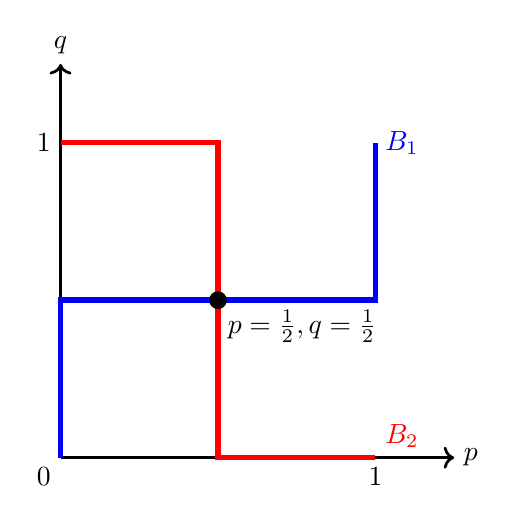
\begin{tikzpicture}[scale=4]
      \draw[line width=1pt, ->] (0,0) -- (0,1.25);
      \draw[line width=1pt, ->] (0,0) -- (1.25,0);

      \draw[line width=2pt, color=blue] (0,0) -- (0,0.5) -- (1,0.5) -- (1,1);
      \draw[line width=2pt, color=red] (0,1) -- (0.5,1) -- (0.5,0) -- (1,0);

      \node[below left] at (0,0) {0};
      \node[left] at (0,1) {1};
      \node[below] at (1,0) {1};

      \node[above] at (0,1.25) {$q$};
      \node[right] at (1.25,0) {$p$};

      \node[right, color=blue] at (1,1) {$B_1$};
      \node[above right, color=red] at (1,0) {$B_2$};

      \node[draw, circle, fill=black, inner sep=0pt, minimum size=6pt] at (0.5,0.5) {};
      \node[below right] at (0.5,0.5) {$p = \frac{1}{2}, q = \frac{1}{2}$};
    \end{tikzpicture}
  \end{center}

  The intersection of $B_1$ and $B_2$ is where they are best responses simultaneously, hence a Nash
  equilibrium.
  In this case, we have $x^1 = (\frac{1}{2}, \frac{1}{2})$ and $x^2 = (\frac{1}{2}, \frac{1}{2})$
  and $(x^1, x^2)$ is an NE.
\end{ex}

\pagebreak
\begin{ex}[Example: Bach or Stravinsky]
  \begin{center}
    \renewcommand{\arraystretch}{1.25}
    \begin{tabular}{c |c|c|}
      \multicolumn{1}{c}{} & \multicolumn{1}{c}{B} & \multicolumn{1}{c}{S} \\
      \cline{2-3}
      B & $2, 1$ & $0, 0$ \\
      \cline{2-3}
      S & $0, 0$, & $2, 1$ \\
      \cline{2-3}
    \end{tabular}
  \end{center}

  Suppose $x^1 = (p, 1 - p)$ and $x^2 = (q, 1 - q)$.

  Then $u_1(B, x^2) = 2q$ and $u_1(S, x^2) = 1 - q$.
  So $u_1(x) = p \cdot 2q + (1 - p) \cdot (1 - q) = p(-1 + 3q) + (1 - q)$.
  Break into cases depending on $q = \frac{1}{3}$.
  The BRF is:
  \[
    B_1(x^2) = \begin{cases}
      \{ (0, 1) \} & \text{if } \ q < \frac{1}{3} \\
      \{ (p, 1 - p) : p \in [0, 1] \} & \text{if } \ q = \frac{1}{3} \\
      \{ (1, 0) \} & \text{if } \ q > \frac{1}{3} \\
    \end{cases}
  \]

  For player II, $u_2(x) = q(-2 + 3p) + 2 - 2p$.
  Break into cases depending on $p = \frac{2}{3}$.
  The BRF is:
  \[
    B_2(x^1) = \begin{cases}
      \{ (0, 1) \} & \text{if } \ p < \frac{2}{3} \\
      \{ (q, 1 - q) : q \in [0, 1] \} & \text{if } \ p = \frac{2}{3} \\
      \{ (1, 0) \} & \text{if } \ p > \frac{2}{3} \\
    \end{cases}
  \]

  The ``graph'' here is:
  \begin{center}
    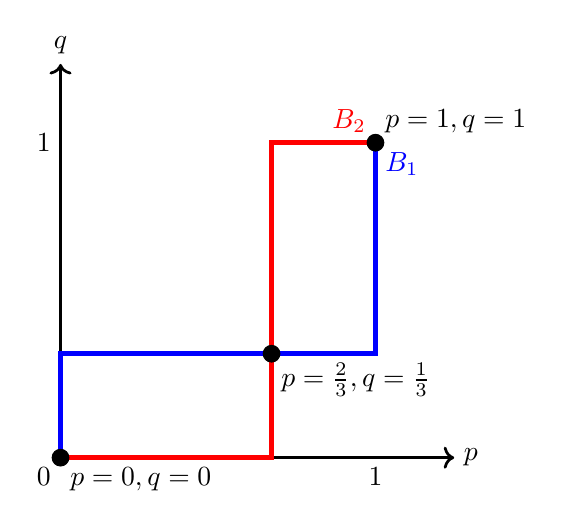
\begin{tikzpicture}[scale=4]
      \draw[line width=1pt, ->] (0,0) -- (0,1.25);
      \draw[line width=1pt, ->] (0,0) -- (1.25,0);

      \draw[line width=2pt, color=blue] (0,0) -- (0,0.33) -- (1,0.33) -- (1,1);
      \draw[line width=2pt, color=red] (0,0) -- (0.67,0) -- (0.67,1) -- (1,1);

      \node[below left] at (0,0) {0};
      \node[left] at (0,1) {1};
      \node[below] at (1,0) {1};

      \node[above] at (0,1.25) {$q$};
      \node[right] at (1.25,0) {$p$};

      \node[below right, color=blue] at (1,1) {$B_1$};
      \node[above left, color=red] at (1,1) {$B_2$};

      \node[draw, circle, fill=black, inner sep=0pt, minimum size=6pt] at (0,0) {};
      \node[below right] at (0,0) {$p = 0, q = 0$};
      \node[draw, circle, fill=black, inner sep=0pt, minimum size=6pt] at (0.67,0.33) {};
      \node[below right] at (0.67,0.33) {$p = \frac{2}{3}, q = \frac{1}{3}$};
      \node[draw, circle, fill=black, inner sep=0pt, minimum size=6pt] at (1,1) {};
      \node[above right] at (1,1) {$p = 1, q = 1$};
    \end{tikzpicture}
  \end{center}

  There are 3 NE here:
  \begin{itemize}
    \item 2 pure strategies: $((0, 1), (0, 1))$ and $((1, 0), (1, 0))$
    \item 1 mixed strategy: $((\frac{2}{3}, \frac{1}{3}), (\frac{1}{3}, \frac{2}{3}))$
  \end{itemize}
\end{ex}

With two players, it is easy to find Nash equilibria; with more players, in general it is not easy.

%%%%% Lec 17
\section{Support Characterization}

Recall: BRF maximizes a player's utility $u_i(x) = \sum\limits_{s \in S_i} x_s^i u_i(s, x^{-i})$.

Suppose $\overline{x}^{-i}$ is fixed.
Which $x^i \in \Delta^i$ maximizes $u_i(x^i, \overline{x}^{-i})$?
Write an LP:

\begin{minipage}{0.9\textwidth}
  \begin{align*}
    \max \quad \sum_{s \in S_i} x_s^i &u_i(s, \overline{x}^{-i}) \\
    \text{s.t.} \quad \sum_{s \in S_i} x_s^i &= 1 \\
    x^i &\geq \mathbb{0} \\
  \end{align*}
\end{minipage}\hfill\begin{minipage}{0.05\textwidth}
  (P)
\end{minipage}

Variables: $x_s^i$ for each $s \in S_i$.
What is the dual?
We have one constraint in (P), so one dual variable $y$.

\begin{minipage}{0.9\textwidth}
  \begin{align*}
    \min \quad y & \\
    \text{s.t.} \quad y &\geq u_i(s, \overline{x}^{-i}) \quad \text{for all } s \in S_i \\
  \end{align*}
\end{minipage}\hfill\begin{minipage}{0.05\textwidth}
  (D)
\end{minipage}

Both (P) and (D) are feasible: for (P), set $x^i$ to any probability distribution; for (D), set $y$
to be the maximum $u_i(s, \overline{x}^{-i})$.
Therefore, (P) and (D) have optimal solutions and their optimal values are equal.

(D) is easy to solve: $y = \max\limits_{s \in S_i} u_i(s, \overline{x}^{-i})$.
This is the maximum utility when pure strategies are played against $\overline{x}^{-i}$.

(P) also has optimal value $y$.
So the maximum utility of all mixed strategies is equal to the max utility of pure strategies.

Complementary slackness conditions: $x_s^i = 0$ or $y = u_i(s, \overline{x}^{-i})$ for all
$s \in S_i$.

Equivalently, $x_s^i > 0$ implies $y = u_i(s, \overline{x}^{-i})$.
Translation: only pure strategies with maximum utility could have positive probabilties in a best
response.

\begin{thm}{support characterization}{17.1}
  Given $\overline{x}^{-i} \in \Delta^{-i}$, a mixed strategy $x^i \in B_i(\overline{x}^{-i})$ if
  and only if $x_s^i > 0$ implies $s \in S_i$ is a pure strategy of maximum utility against
  $\overline{x}^{-i}$.
\end{thm}

\begin{defn}{support}{support}
  For a mixed strategy $x^i \in \Delta^i$, the \hldef{support} is the set of strategies with
  positive probability in $x^i$.
\end{defn}

Rephrasing \cref{thm:17.1}: $x^i$ is in the BRF if and only if the support of $x^i$ are strategies
with maximum utility.

\begin{ex}[Example: Bach or Stravinsky]
  \begin{center}
    \renewcommand{\arraystretch}{1.25}
    \begin{tabular}{c |c|c|}
      \multicolumn{1}{c}{} & \multicolumn{1}{c}{B} & \multicolumn{1}{c}{S} \\
      \cline{2-3}
      B & $2, 1$ & $0, 0$ \\
      \cline{2-3}
      S & $0, 0$, & $2, 1$ \\
      \cline{2-3}
    \end{tabular}
  \end{center}

  Suppose player II plays $x^2 = (q, 1 - q)$.
  The utilities of player I using pure strategies are $u_1(\text{B}, x^2) = 2q$ and
  $u_1(\text{S}, x^2) = 1 - q$.
  Depending on $q$, the strategies with maximum utility are different.
  \begin{enumerate}
    \item
    If $2q < 1 - q$, then $q < \frac{1}{3}$, and B is not in the support and gets probability 0.
    BRF is $\{(0, 1)\}$.
    \item
    If $2q = 1 - q$, then $q = \frac{1}{3}$, and both B and S could be in the support.
    Any combination works, so BRF is $\{(p, 1 - p) : p \in [0, 1]\}$.
    \item
    If $2q > 1 - q$, then $q > \frac{1}{3}$, and S is not in the support and gets probability 0.
    BRF is $\{(1, 0)\}$.
  \end{enumerate}
  This matches the BRF we calculated in the last lecture.
\end{ex}

\begin{ex}
  Consider a 2-player game with this payoff table:
  \begin{center}
    \renewcommand{\arraystretch}{1.25}
    \begin{tabular}{c |c|c|c|}
      \multicolumn{1}{c}{} & \multicolumn{1}{c}{D} & \multicolumn{1}{c}{E}
        & \multicolumn{1}{c}{F} \\
      \cline{2-4}
      A & $2, 2$ & $3, 3$ & $1, 1$ \\
      \cline{2-4}
      B & $3, 1$ & $0, 4$ & $2, 1$ \\
      \cline{2-4}
      C & $3, 4$, & $5, 1$ & $0, 7$ \\
      \cline{2-4}
    \end{tabular}
  \end{center}

  Suppose player II plays $x^2 = (0, \frac{1}{3}, \frac{1}{2})$.
  What is $B_1(x^2)$?
  \begin{itemize}
    \item $u_1(A, x^2) = 0 \cdot 2 + \frac{1}{3} \cdot 3 + \frac{2}{3} \cdot 1 = \frac{5}{3}$
    \item $u_1(B, x^2) = 0 \cdot 3 + \frac{1}{3} \cdot 0 + \frac{2}{3} \cdot 2 = \frac{4}{3}$
    \item $u_1(C, x^2) = 0 \cdot 3 + \frac{1}{3} \cdot 5 + \frac{2}{3} \cdot 0 = \frac{5}{3}$
  \end{itemize}
  Playing A or C gives the maximum utility.
  By support characterization, $x_B^1 = 0$.
  Any distribution over $x_A^1$ and $x_C^1$ works.

  The BRF is $B_1(x^2) = \{ (p, 0, 1 - p) : p \in [0, 1] \}$.

  The maximum utility for player I is
  $p \cdot \frac{5}{3} + (1 - p) \cdot \frac{5}{3} = \frac{5}{3}$, which is equal to the maximum
  utility for a pure strategy.

  Any strategy in $B_1(x^2)$ maximizes utility for player I.
  Which of these maximizes utility for player II?
  This will give a Nash equilibrium.

  Suppose $x^1 = (p, 0, 1 - p)$.
  Then:
  \begin{itemize}
    \item $u_2(D, x^1) = 4 - 2p$
    \item $u_2(E, x^1) = 1 + 2p$
    \item $u_2(F, x^1) = 7 - 6p$
  \end{itemize}
  If $x^2 = (0, \frac{1}{3}, \frac{2}{3})$ is in the best response, then E and F must have (the
  same) maximum utility.
  That is, $1 + 2p = 7 - 6p$ so $p = \frac{3}{4}$.
  The utility for E and F is then $\frac{5}{2}$; the utility for D is also $\frac{5}{2}$, so E and F
  indeed have maximum utility.
  (So does D, but this is fine.)

  So $x^1 = (\frac{3}{4}, 0, \frac{1}{4})$ and $x^2 = (0, \frac{1}{3}, \frac{2}{3})$ are best
  responses to each other, and $(x^1, x^2)$ is a Nash equilibrium.
\end{ex}

Note: one ``algorithm'' for finding an NE is by looking at possible combinations of the supports for
each player.
In the example above, if we say ``suppose player I's support is \{\text{A}, \text{C}\} and player
II's support is \{\text{E}, \text{F}\}'' then we can use support characterization to find an NE or
prove none exist for these supports.
Problem: this grows exponentially ($~2^k$ possible supports for each player if there are $k$ pure
strategies), so it is not practical.

\begin{exer}{}{17.2}
  Show that in the game of rock paper scissors, both players playing $(\frac{1}{3}, \frac{1}{3},
  \frac{1}{3})$ is the only Nash equilibrium.
\end{exer}

%%%%% Lec 18
\section{Voting Game}

Downs paradox: Voting has costs.
The probability that one vote is a decisive vote is very small.
Costs outweigh benefits.

Expectation: people don't vote.
Reality: people do vote.

Model for voter participation: Suppose there are candidates $A, B$ and the number of supporters are
$a, b$, respectively.
WLOG, assume $a \geq b$.
Each person can choose to ``vote'' or ``abstain''.
If they vote, then they incur a cost of $c$ where $0 < c < 1$.
Regardless of voting or abstaining, each person gets a payoff of 2 if their supporting candidate
wins, 1 for a tie, or 0 for a loss.

\subsection{Pure Nash equilibria}

Suppose $a = b = 1$.
\begin{center}
  \renewcommand{\arraystretch}{1.25}
  \begin{tabular}{c c|c|c|}
    \multicolumn{2}{c}{} & \multicolumn{2}{c}{P II (B)} \\
    \multicolumn{2}{c}{} & \multicolumn{1}{c}{A} & \multicolumn{1}{c}{V} \\
    \cline{3-4}
    \multirow{2}{*}{P I (A)} & A & $1, 1$ & $0, 2 - c$ \\
    \cline{3-4}
    & V & $2 - c, 0$, & $1 - c, 1 - c$ \\
    \cline{3-4}
  \end{tabular}
\end{center}
This is similar to prisoner's dilemma: if both players vote, they get lower utility than if both
players abstain.
(Both voting is an NE.)

Suppose $a = b \geq 2$.
There are 4 cases:
\begin{enumcase}
  \item
  Everyone votes.

  Tie: everyone has utility $1 - c$, switching gives $0$.
  NE.
  \item
  Not everyone votes, but there is a tie.

  One who abstains can vote, moving utility from $1$ to $2 - c > 1$.
  Not NE.
  \item
  One candidate wins by 1 vote.

  One who abstains for the loser can vote, moving utility from $0$ to $1 - c > 0$.
  Not NE.
  \item
  One candidate wins by at least 2 votes.

  One for votes for the winning candidate can abstain, moving utility from $2 - c$ to $2 > 2 - c$.
  Not NE.
\end{enumcase}
In a close election, we expect more people to vote.

\begin{exer}{}{18.1}
  Show that when $a > b$, there is no pure Nash equilibrium.
\end{exer}

\subsection{Mixed Nash equilibria}

One possible scenario for a mixed NE.

Suppose $a > b$.
Suppose among all $A$ supporters, $b$ of them will vote and $a - b$ of them will abstain.
Suppose every $B$ supporter will vote with the same probability $p$.
So the best that $B$ can do is a tie.
It is easy to check that $p = 0$ or $p = 1$ is not an NE.
Assume $p \in (0, 1)$.

Consider a $B$ supporter.
If they abstain, then $B$ cannot win.
So utility of ``abstain'' as a pure strategy is 0.
If they vote, then $B$ ties only if all other $B$ supporters vote (utility $1 - c$), otherwise $B$
loses (utility $-c$).
The expected utility of ``vote'' as a pure strategy is
$p^{b - 1} (1 - c) + (1 - p^{b - 1}) (-c) = p^{b - 1} - c$.

When is it possible that this is in an NE?
$p \in (0, 1)$, so both strategies have positive probabilities.
To be in the best response, support characterization implies that the two utilities are equal.
So $0 = p^{b - 1} - c$, or $p = c^{\frac{1}{b - 1}}$.

Given this $p$, are $A$ supporters incentivized to change their mixed strategies?
Currently, all of them are playing pure strategies.
In order to switch, the utility of switching to the other pure strategy must be greater.

\begin{enumcase}
  \item
  Consider an $A$ supporter who abstained.
  Expected utility is $p^b \cdot 1 + (1 - p^b) \cdot 2 = 2 - p^b$.

  Expected utility of voting is $2 - c$ ($A$ is guaranteed to win).
  $2 - c = 2 - p^{b - 1} \leq 2 - p^b$ since $0 < p < 1$.
  Switching to a pure strategy does not increase utility.
  So switching to any mixed strategy does not increase utility.
  There is no reason to switch.
  \item
  Consider an $A$ supporter who voted.
  Expected utility is $p^b \cdot (1 - c) + (1 - p^b) \cdot (2 - c) = 2 - p^b - c$.

  If they abstain, then $A$ loses if all $B$ supporters vote, $A$ ties if $b - 1$ $B$ supporters
  vote, or $A$ wins otherwise.
  The expected utility of abstaining is $p^b \cdot 0 + b \cdot p^{b - 1} \cdot (1 - p) \cdot 1 +
    (1 - p^b - b \cdot p^{b - 1} \cdot (1 - p)) \cdot 2 = 2 - 2p^b - b p^{b - 1} (1 - p)$.
  Check: $2 - p^b - c \geq 2 - 2p^b - b p^{b - 1} (1 - p)$.
  There is no reason to switch.
\end{enumcase}

When $p = c^{\frac{1}{b - 1}}$, this is a mixed NE.

What happens to voter participation as cost increases?
If $c$ increases, then $p$ increases, so more voters will vote.

%%%%% Lec 19
\section{Two-player Zero-sum Games}

\begin{defn}{zero-sum game}{zero_sum_game}
  A strategic game is a \hldef{zero-sum game} if for all strategy profiles $s \in S$,
  $\sum\limits_{i \in N} u_i(s) = 0$.
\end{defn}

Examples: matching pennies and rock paper scissors.

For a two-player zero-sum game, let $S_1 = \{ 1, \ldots, m \}$ and $S_2 = \{ 1, \ldots, n \}$.
Define such a game with a payoff matrix $A \in \mathbb{R}^{m \times n}$ where $u_1(i, j) = A_{ij}$
and $u_2(i, j) = -A_{ij}$.

\begin{ex}
  Payoff for player I:
  \begin{center}
    \renewcommand{\arraystretch}{1.25}
    \begin{tabular}{c c |c|c|c|c}
      \multicolumn{2}{c}{} & \multicolumn{3}{c}{P II} & \\
      \multicolumn{2}{c}{} & \multicolumn{1}{c}{1} & \multicolumn{1}{c}{2}
        & \multicolumn{1}{c}{3} & \\
      \cline{3-5}
      \multirow{2}{*}{P I} & 1 & 3 & 5 & $-2$ & \multirow{2}{*}{= $A$} \\
      \cline{3-5}
      & 2 & $-5$ & 7 & 1 & \\
      \cline{3-5}
    \end{tabular}
  \end{center}
  Payoff for player II is $-A$.
\end{ex}

Note: for a mixed strategy profile $x = (x^1, x^2)$, we have $u_1(x^1, x^2) = -u_2(x^1, x^2)$.

\subsection{Min-maxing argument for finding a Nash equilibrium}

Given a strategy that we play, the opposing player will maximize their utility, which minimizes our
utility.
Knowing how they would play, what can we do to maximize our own utility?

Player I's perspective: Suppose player I plays $x^1$.
They expect player II to play from their best response.

\begin{ex}
  The expected utilities for player II's 3 strategies above are $u_2(1, x^1) = -3x_1^1 + 5x_2^1$,
  $u_2(2, x^1) = -5x_1^1 - 7x_2^1$, and $u_3(3, x^1) = 2x_1^1 - x_2^1$.

  We look for
  \begin{align*}
    & \max \{ -3x_1^1 + 5x_2^1, -5x_1^1 - 7x_2^1, 2x_1^1 - x_2^1 \} \\
    =& \min \{ 3x_1^1 - 5x_2^1, 5x_1^1 + 7x_2^1, -2x_1^1 + x_2^1 \}.
  \end{align*}

  We wish to maximize:
  \begin{align*}
    \max \quad & u_1 \\
    \text{s.t.} \quad & u_1 \leq 3x_1^1 - 5x_2^1 \\
    & u_1 \leq 5x_1^1 + 7x_2^1 \\
    & u_1 \leq -2x_1^1 + x_2^1 \\
    & x_1^1 + x_2^1 = 1 \\
    & x_1 \geq \mathbb{0}
  \end{align*}
\end{ex}

Player II's expected utility for playing pure strategy $j$ is $-(x^1)^T A_{\bullet j}$ (where
$A_{\bullet j}$ is the $j$-th column of $A$).
The utility of player II's best response is equal to the maximum of these values:
\[
  \max_{j \in \{1, \ldots, n\}} -(x^1)^T A_{\bullet j}
    = -\min_{j \in \{1, \ldots, n\}} (x^1)^T A_{\bullet j}.
\]
So utility for player I is $\min\limits_{j \in \{1, \ldots, n\}} (x^1)^T A_{\bullet j}$.
Player I wants to maximize this.

\begin{center}
\begin{tabular}{c c c}
  $\begin{aligned}
    \max \quad & \min_{j \in \{1, \ldots, n\}} (x^1)^T A_{\bullet j} \\
    \text{s.t.} \quad & \sum_{i = 1}^m x_i^1 = 1 \\
    & x_1 \geq \mathbb{0} \\
  \end{aligned}$
  &
  $\longrightarrow$
  &
  $\begin{aligned}
    \max \quad & u_1 \\
    \text{s.t.} \quad & u_1 \leq (x^1)^T A_{\bullet j} \ \forall j \in \{1, \ldots, n\} \\
    & \sum_{i = 1}^m x_i^1 = 1 \\
    & x^1 \geq \mathbb{0}
  \end{aligned}$
  \\
\end{tabular}
\end{center}

Player II's perspective: Suppose player II plays $x^2$.
Then player I will play from their best response.

\begin{ex}
  Player I's best response has utility
  \[
    \max\{ 3x_1^2 + 5x_2^2 - 2x_3^2, -5x_1^2 + 7x_2^2 + x_3^2 \}.
  \]

  We wish to minimize:
  \begin{align*}
    \min \quad & u_2 \\
    \text{s.t.} \quad & 3x_1^2 + 5x_2^2 - 2x_3^2 \leq u_2 \\
    & {-}5x_1^2 + 7x_2^2 + x_3^2 \leq u_2 \\
    & x_1^2 + x_2^2 + x_3^2 = 1 \\
    & x_2 \geq \mathbb{0}
  \end{align*}
\end{ex}

The utility of player I's best response is
$\max\limits_{i \in \{1, \ldots, m\}} (x^2)^T A_{i \bullet}$ (where $A_{i \bullet}$ is the $i$-th
row of $A$).
Player II's utility is $-\max\limits_{i \in \{1, \ldots, m\}} (x^2)^T A_{i \bullet}$.
Maximizing this is equivalent to minimizing
$\max\limits_{i \in \{1, \ldots, m\}} (x^2)^T A_{i \bullet}$:

\begin{center}
\begin{tabular}{c c c}
  $\begin{aligned}
    \max \quad & \min_{i \in \{1, \ldots, m\}} (x^2)^T A_{i \bullet} \\
    \text{s.t.} \quad & \sum_{j = 1}^n x_j^2 = 1 \\
    & x_2 \geq \mathbb{0} \\
  \end{aligned}$
  &
  $\longrightarrow$
  &
  $\begin{aligned}
    \max \quad & u_2 \\
    \text{s.t.} \quad & u_2 \leq (x^2)^T A_{i \bullet} \ \forall i \in \{1, \ldots, m\} \\
    & \sum_{j = 1}^n x_j^2 = 1 \\
    & x^2 \geq \mathbb{0}
  \end{aligned}$
  \\
\end{tabular}
\end{center}

Main result: the LPs for player I and player II are duals of each other.
(Exercise: verify this in general.)

Both LPs are feasible (take $x^1, x^2$ to be any probability distributions and $u_1, u_2$ as
max/min values).
So both have optimal solutions with the same objective value.
(Note: objective value of player I's LP is the utility of player I, so the objective value of
player II's LP is the negative of the utility of player II.)
The optimal solutions are best responses to each other, so they form a Nash equilibrium.
Solve for this using simplex (a modified version of simplex is provably polynomial time).

\begin{thm}{}{19.1}
  Any (finite) two-player zero-sum game has a mixed Nash equilibrium, and this can be efficiently
  computed.
\end{thm}

\begin{ex}
  For our two LPs above, an optimal solution is
  \begin{itemize}
    \item Player I: $x^1 = (\frac{6}{11}, \frac{5}{11})$ and $u_1 = \frac{-7}{11}$
    \item Player II: $x^2 = (\frac{3}{11}, 0, \frac{8}{11})$ and $u_2 = \frac{-7}{11}$
  \end{itemize}
  where player I's utility is $u_1$ and player II's utility is $-u_2$.
\end{ex}

Note: computing NEs in general is difficult.
Even in the 3-player zero-sum game or 2-player general-sum game, no polynomial time algorithm is
known.

%%%%% Lec 20
\section{Nash's Theorem (I)}

\begin{thm}{Nash's theorem}{20.1}
  Every strategic game with finitely many players and pure strategies has a Nash equilibrium.
\end{thm}

\subsection{Brouwer's fixed point theorem}

\begin{thm*}{Brouwer's fixed point theorem}
  Let $X$ be a convex and compact set in a finite-dimensional Euclidean space, and let
  $f \colon X \to X$ be a continuous function.
  Then there exists $x_0 \in X$ such that $f(x_0) = x_0$ (``fixed point'').
\end{thm*}

\begin{ex}
  Let $X = [0, 1]$.
  Consider any continuous function $f \colon [0, 1] \to [0, 1]$.

  \begin{center}
    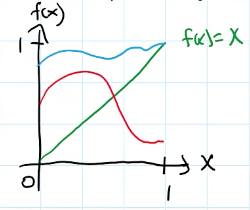
\includegraphics[width=0.3\textwidth]{20-1}
  \end{center}

  The graph of $f$ will always intersect $f(x) = x$, producing a fixed point.
  This is a consequence of the intermediate value theorem (applied to $f(x) - x$).
\end{ex}

Terminology from the theorem:
\begin{itemize}
  \item
  We will think of a Euclidean space as $\mathbb{R}^n$ with the standard dot product, which defines
  how we measure distance and angle.
  \item
  A set is convex if for any two points in the set, the line segment joining them is also in the
  set.
  Precise definition: $S$ is convex if for all $u, v \in S$, $\lambda u + (1 - \lambda) v \in S$ for
  all $\lambda \in [0, 1]$.
  Note that the convex combination of any set of points is convex:
  $S = \{ \lambda_1 v_1 + \cdots + \lambda_n v_n : \lambda_1, \ldots, \lambda_n \geq 0,
    \lambda_1 + \cdots + \lambda_n = 1 \}$ is convex.
  \item
  A set is compact if it is closed and bounded.
  Closed: all ``boundary'' points are in the set, \emph{e.g.} $[0, 1]$ is closed, $(0, 1)$ is not
  closed.
  Bounded: there is a constant that bounds the distance between any two points.
\end{itemize}

Note: this is a deep theorem from analysis.
We will not prove it here, though there are many fascinating proofs of it (suggestion: look into the
combinatorial proof using Sperner's Lemma).
None of the proofs are constructive: we know that a fixed point exists, but the proofs do not tell
us how to find one.

Illustrations:
\begin{enumerate}
  \item
  Print a world map and place it on your desk.
  This is a continuous mapping from the surface of the Earth to the part of the surface occupied by
  the map on your desk.
  The theorem implies there is a fixed point: some point on the map is directly on top of the point
  it represents on your desk.
  \item
  Take a cup of tea and stir it.
  Let it settle.
  Then some part of the liquid is in the same spot before the stir.
\end{enumerate}

\subsection{Relation to strategic games}

We want to use Brouwer's fixed point theorem when $X$ is the set of all mixed strategy profiles of
a finite strategic game.
Need to verify that $\Delta$ is convex and compact.

Start with just one player $i$ and their set of mixed strategies $\Delta^i$.
If the set of pure strategies is $\{1, \ldots, k\}$, then
\[
  \Delta^i = \{ (x_1^i, \ldots, x_k^i) : x_j^i \geq 0, x_1^i + \cdots + x_k^i = 1 \}.
\]

\begin{minipage}[t]{0.4\textwidth}
  $k = 2$: $\Delta^i = \{(p, 1 - p) : p \in [0, 1]\}$

  \vspace{\baselineskip}
  \begin{center}
    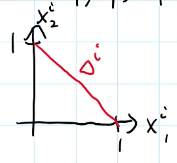
\includegraphics[width=4.5cm]{20-2}
  \end{center}
\end{minipage}\hfill\begin{minipage}[t]{0.55\textwidth}
  $k = 3$: $\Delta^i = \{(p, q, r) : p + q + r = 1, p, q, r \geq 0\}$

  \vspace{\baselineskip}
  \begin{center}
    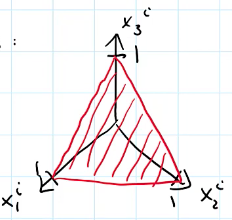
\includegraphics[width=4.5cm]{20-3}
  \end{center}
\end{minipage}

We can see (without proof) that $\Delta^i$ is compact: it is closed, and any 2 points have distance
at most $\sqrt{2}$.
$\Delta^i$ is convex: it is the convex combination of the standard basis vectors $e_1, \ldots, e_k$.
(An element of $\Delta^i$ has the form $x_1^i e_1 + \cdots + x_k^i e_k$ where
$x_1^i + \cdots + x_k^i = 1$, $x_j^i \geq 0$.)
These $e_1, \ldots, e_k$ are the pure strategies of player $i$.

The set of all strategy profiles is $\Delta = \Delta^1 \times \cdots \times \Delta^n$.
We can ``pretend'' that this is a set in $\mathbb{R}^{\abs{S_1} + \cdots + \abs{S_n}}$.
It is still compact (a result from analysis is that the cartesian product of compact sets is
compact).
It is also convex (exercise).
So we can use $\Delta$ as the set in Brouwer's fixed point theorem.

To do: find a continuous function $f \colon \Delta \to \Delta$ that relates fixed points to Nash
equilibria.

%%%%% Lec 21
\section{Nash's Theorem (II)}

Recall: the set of all strategy profiles $\Delta$ is convex and compact.
Need $f \colon \Delta \to \Delta$ to relate fixed points and Nash equilibria.

\subsection{Main idea}

Given a strategy profile $x = (x^1, \ldots, x^n)$, a player $i$ will look at possibly switching to a
pure strategy to gain utility against $x^{-i}$.
If pure strategy $s$ improves utility, then player $i$ wants to shift the probability distribution
so that $s$ receives higher probability.
The function will take $x$ and map it to another strategy profile where each player improves their
utility.

\begin{ex}[Example: rock paper scissors]
  Suppose both play rock as a pure strategy.
  They can increase utility by moving toward paper.
  \begin{center}
    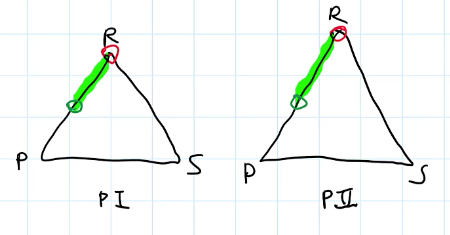
\includegraphics[width=0.45\textwidth]{21-1}
  \end{center}
  Suppose player I plays rock and player II plays paper.
  Player II cannot improve utility.
  Player I can improve utility by 1 if they move to paper, or improve utility by 2 if they move to
  scissors.
  Player I will move more toward scissors than paper.
  \begin{center}
    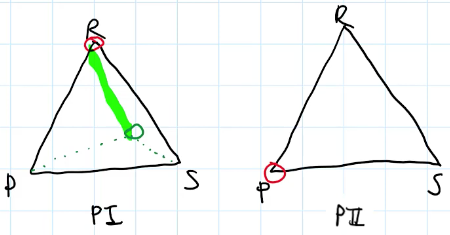
\includegraphics[width=0.45\textwidth]{21-2}
  \end{center}
\end{ex}

What is the meaning of a fixed point?
No player can improve their utility.
So it must be a Nash equilibrium.

\subsection{Defining the function}

First, define $\Phi$ which records the improvement of a player in switching to a pure strategy.
Given strategy profile $x \in \Delta$, a player $i$, and a pure strategy $s \in S_i$, define
\[
  \Phi_s^i(x) = \max \{ 0, u_i(s, x^{-i}) - u_i(x) \}.
\]
If playing $s$ increases utility for player $i$, then $\Phi_s^i(x)$ represents this increase;
otherwise $\Phi_s^i(x) = 0$.

For player $i$ and strategies $s$ where $\Phi_s^i(x) > 0$, we want to increase the probability
assigned to $s$.
We want to replace $x_s^i$ by $x_s^i + \Phi_s^i(x)$, but the sum of the probabilities would be
greater than 1.
We can normalize this by dividing by $\sum\limits_{s' \in S_i} (x_{s'}^i + \Phi_{s'}^i(x)) =
  1 + \sum\limits_{s' \in S_i} \Phi_{s'}^i(x)$.

We define $f \colon \Delta \to \Delta$ by $f(x) = \overline{x}$ where for each player $i$ and
strategy $s \in S_i$,
\[
  \overline{x}_s^i = \frac{x_s^i + \Phi_s^i(x)}{1 + \sum\limits_{s' \in S_i} \Phi_{s'}^i(x)}.
\]
Verify that $f(x) \in \Delta$.

\begin{ex}
  In rock paper scissors where player I plays rock and player II plays paper, the strategy profile
  is $x = ((1, 0, 0), (0, 1, 0))$.
  For player II, $\Phi_s^2(x) = 0$ for each $s \in \{ \text{R}, \text{P}, \text{S} \}$.
  For player I, $\Phi_\text{R}^1(x) = 0$, $\Phi_\text{P}^1(x) = 1$, and $\Phi_\text{S}^1(x) = 2$.
  So the new strategy for player I is
  \[
    \overline{x}_\text{R}^1 = \frac{1 + 0}{1 + 3} = \frac{1}{4}, \quad
    \overline{x}_\text{P}^1 = \frac{0 + 1}{1 + 3} = \frac{1}{4}, \quad
    \overline{x}_\text{S}^1 = \frac{0 + 2}{1 + 3} = \frac{1}{2}.
  \]
  Then $f(x) = ((\frac{1}{4}, \frac{1}{4}, \frac{1}{2}), (0, 1, 0))$.
\end{ex}

\subsection{Completing the proof of Nash's theorem}

Given $x \in \Delta$, consider $\Phi$ and $f \colon \Delta \to \Delta$ defined above.
We see that $f$ is continuous since $\Phi$ is continuous.
By Brouwer's fixed point theorem, there exists $\hat{x} \in \Delta$ such that
$f(\hat{x}) = \hat{x}$.
We prove that $\hat{x}$ is a NE by showing $\hat{x}^i \in B_i(\hat{x}^{-i})$.

For player $i$, let $s \in S_i$ be a pure strategy such that $\hat{x}_s^i > 0$ and
$u_i(s, \hat{x}^{-i}) \leq u_i(\hat{x})$.
(Exercise: show such $s$ exists.)
Then $\Phi_s^i(\hat{x}) = 0$.
Since $\hat{x}$ is a fixed point, $\hat{x}_s^i = (f(\hat{x}))_s^i =
  \hat{x}_s^i / (1 + \sum\limits_{s' \in S_i} \Phi_{s'}^i (\hat{x}))$.
Since $\hat{x}_s^i > 0$, the denominator must be 1.
So $\sum\limits_{s' \in S_i} \Phi_{s'}^i(\hat{x}) = 0$.
But $\Phi$ is non-negative, so $\Phi_{s'}^i(\hat{x}) = 0$ for all $s' \in S_i$.
This means that $u_i(s', \hat{x}^{-i}) \leq u_i(\hat{x})$ for all $s' \in S_i$.
So playing $\hat{x}^i$ gives the highest utility against $\hat{x}^{-i}$, so
$\hat{x}^i \in B_i(\hat{x}^{-i})$.
Since this holds for all players, $\hat{x}$ is a Nash equilibrium.
\hfill $\qed$

Note: this proves that a NE always exists, but the proof does not show us how to find such a NE, as
it depends on Brouwer's fixed point theorem.

%%%%% Topic: Cooperative Games
\coursetopic{Cooperative Games}

%%%%% Lec 22
\section{Cooperative Games}

There are games where groups of players can work together to obtain higher utility.

\begin{ex}
  Alice (A), Bob (B), and Carol (C) want to buy ice cream.
  There are three sizes of ice cream: 1L, 1.5L, and 2L with costs \$7, \$9, \$11 respectively.
  A has \$3, B has \$4, C has \$5.
  On their own, they cannot buy any.
  But if they pool money together, they can get some ice cream.
  (For example, B + C can buy 1.5L.)
\end{ex}

\begin{defn}{cooperative game}{cooperative_game}
  A \hldef{cooperative game} is given by a set of players $N$ and a characteristic function
  $v \colon 2^N \to \mathbb{R}$ that assigns a value $v(S)$ to each coalition $S \subseteq N$ of
  players.
  We use $(N, v)$ to represent this game.
  The set $N$ is the \hldef{grand coalition}.
\end{defn}

\begin{ex}
  In the ice cream game, $N = \{ \text{A}, \text{B}, \text{C} \}$ and $v$ is defined by:
  \[
    \begin{array}{c|c|c|c|c|c}
      S & \varnothing, \{\text{A}\}, \{\text{B}\}, \{\text{C}\} & \{\text{A}, \text{B}\}
        & \{\text{A}, \text{C}\} & \{\text{B}, \text{C}\} & \{\text{A}, \text{B}, \text{C}\} \\
      \hline
      v(S) & 0 & 1 & 1 & 1.5 & 2 \\
    \end{array}
  \]
\end{ex}

General assumptions: $v(\varnothing) = 0$, $v(S) \geq 0$ for all $S \subseteq N$.

\begin{ex}
  A country has 101-member parliament.
  There are 4 parties A, B, C, D with 40, 22, 30, 9 members, respectively.
  They need to decide how to spend a \$1B winfall but they need to form a majority to spend it.
  \[
    N = \{A, B, C, D\}, \qquad v(S) = \begin{cases}
      10^9 & \text{if parties in } S \text{ have at least 51 members} \\
      0 & \text{otherwise}
    \end{cases}
  \]
\end{ex}

\begin{ex}
  In a matching game, we are given a graph $G = (V, E)$ and edge weights
  $w \colon E \to \mathbb{R}$.
  The players are the vertices, $V = N$.
  The weight of an edge represents the benefits if the two vertex players work together.
  For any subset $S \subseteq N$, the value is the maximum weight of a matching using vertices in
  $S$.
\end{ex}

\subsection{Outcomes of cooperative games}

Outcomes of strategic games: strategy profiles (pure or mixed).
Which strategy is played by each player?

Outcomes of cooperative games:
\begin{enumerate}
  \item
  Divide the players into groups, called coalitions (``coalition structure'').
  Each coalition will generate their assigned value.
  \item
  Distribute the value that each coalition generates among its members (``payoff vector'').
\end{enumerate}

\begin{defn}{coalition structure, payoff vector, efficient}{cooperative_defns}
  Given a cooperative game $(N, v)$, a \hldef{coalition structure} is a partition $\pi$ of $N$,
  \emph{i.e.} $\pi = (C^1, \ldots, C^k)$ where each $C^i \subseteq N$, $C^i \cap C^j = \varnothing$
  whenever $i \neq j$, and $C^1 \cup \cdots \cup C^k = N$.

  A \hldef{payoff vector} is a vector $x \in \mathbb{R}^N$ such that $x \geq \mathbb{0}$ and
  $\sum\limits_{i \in C^j} x_i \leq v(C^j)$ for all $j = 1, \ldots, k$.

  Notation: for any $T \subseteq N$, $x(T) = \sum\limits_{i \in T} x_i$.
  So the inequality here is $x(C_j) \leq v(C^j)$.

  An outcome consists of $(\pi, x)$.
  Such an outcome is \hldef{efficient} if $x(C^j) = v(C^j)$ for all $j$.
\end{defn}

\begin{ex}
  An outcome of the ice cream game is $(\pi, x)$ where
  $\pi = (\{\text{A}, \text{B}\}, \{\text{C}\})$ and $x_\text{A} = 0.5$, $x_\text{B} = 0.5$, and
  $x_\text{C} = 0$.
  This outcome is efficient: $v(\{\text{A}, \text{B}\}) = 1 = x_\text{A} + x_\text{B}$ and
  $v(\{\text{C}\}) = x_\text{C}$.
\end{ex}

\pagebreak
\subsection{Some classes of games}

\begin{enumerate}
  \item
  \hldef{Monotone games}: $S \subseteq T \implies v(S) \leq v(T)$ (``more people produce more
  value'').
  \item
  \hldef{Superadditive games}: for disjoint $S, T$, $v(S) + v(T) \leq v(S \cup T)$ (``forming
  coalitions is always better'').

  Superadditivity implies monotonicity, but the converse is not true.
  We usually only consider the grand coalition: $\pi = (N)$.
  \item
  \hldef{Convex games}: for any $S, T$, $v(S) + v(T) \leq v(S \cup T) + v(S \cap T)$
  (supermodularity inequality).

  Convexity implies superadditivity, but the converse is not true.
\end{enumerate}

\begin{prop}{}{21.1}
  A game $(N, v)$ is convex if and only if for every $S, T$ where $S \subseteq T \subseteq N$ and
  for every player $i \in N \setminus T$, $v(T \cup \{i\}) - v(T) \geq v(S \cup \{i\}) - v(S)$.
\end{prop}

(Proof as exercise.)

This proposition gives the intuition ``a player is more useful in larger coalitions''.

%%%%% Lec 23
\section{Shapley Values (I)}

Two desirable properties of an outcome in cooperative games:
\begin{enumerate}
  \item
  Fairness.
  The payoff vector should reflec the contribution of the playres to their coalitions.
  \item
  Stability.
  We want to incentivize the players to stay in their assigned coalition in the coalition structure.
\end{enumerate}

\subsection{Shapley values}

Shapley values deal with the fairness of the payoff vector.
Assume players form the grand coalition.
(If not, look at individual coalitions separately.)

Question: how can we quantify a player's contribution?

Idea 1: compare the value of the coalition before and after a player joins it.

\begin{ex}
  In the ice cream game, the contribution of A is
  $v(\{\text{A}, \text{B}, \text{C}\}) - v(\{\text{B}, \text{C}\}) = 0.5$.
  The contribution of B is 1 and the contribution of C is 1.

  Can a payoff vector take these values?
  No.
\end{ex}

Problem: the sum of the payoffs may exceed the value of the coalition ($x(N) > v(N)$).

Idea 2: fix a sequence of the players and see their contribution sequentially.

\begin{ex}
  Consider the ice cream game with sequence A, B, C.
  $v(\{\text{A}\}) = 0$, so A contributes 0.
  $v(\{\text{A}, \text{B}\}) = 1$, so B contributes 1.
  $v(\{\text{A}, \text{B}, \text{C}\}) = 2$, so C contributes 1.

  This is efficient: $x(N) = v(N)$.
\end{ex}

Problem: different ordering produce different results.

Shapley's idea: look at all possible orderings of players and average a player's contributions.

Notation:
\begin{itemize}
  \item
  A permutation of $N$ has the form $\sigma = (\sigma_1, \ldots, \sigma_n)$ where each $\sigma_1$ is
  a distinct element of $N$.
  \item
  The element $\sigma_i$ is at the $i$-th position of $\sigma$.
  \item
  The set of all permutations of $N$ is denoted $S_N$.
\end{itemize}

\begin{defn}{marginal contribution, Shapley value}{shapley_defns}
  Given a permutation $\sigma \in S_N$, the \hldef{marginal contribution} of player $\sigma_i$ is
  $\Delta_\sigma(\sigma_i) = v(\{\sigma_1, \ldots, \sigma_i\}) -
    v(\{\sigma_1, \ldots, \sigma_{i - 1}\})$.

    The \hldef{Shapley value} of player $i$ is
    \[
      \varphi_i = \frac{1}{n!} \sum_{\sigma \in S_N} \Delta_\sigma(i).
    \]
\end{defn}

\begin{ex}
  In the ice cream game, $N = \{\text{A, B, C}\}$ and six permuations:
  \[
    \renewcommand{\arraystretch}{1.2}
    \begin{array}{cc}
      \sigma^1 = (\text{A}, \text{B}, \text{C})
      & \sigma^4 = (\text{B}, \text{C}, \text{A}) \\
      \sigma^2 = (\text{A}, \text{C}, \text{B})
      & \sigma^5 = (\text{C}, \text{A}, \text{B}) \\
      \sigma^3 = (\text{B}, \text{A}, \text{C})
      & \sigma^6 = (\text{C}, \text{B}, \text{A}) \\
    \end{array}
  \]
  We calculate the marginal contribution of A in each of the permutations:
  \[
    \renewcommand{\arraystretch}{1.2}
    \begin{array}{ll}
      \Delta_{\sigma^1}(\text{A}) = v(\{\text{A}\}) - v(\varnothing) = 0
      & \Delta_{\sigma^4}(\text{A}) = v(\{\text{B}, \text{C}, \text{A}\})
        - v(\{\text{B}, \text{C}\}) = 0.5 \\
      \Delta_{\sigma^2}(\text{A}) = v(\{\text{A}\}) - v(\varnothing) = 0
      & \Delta_{\sigma^5}(\text{A}) = v(\{\text{C}, \text{A}\}) - v(\{\text{C}\}) = 1 \\
      \Delta_{\sigma^3}(\text{A}) = v(\{\text{B}, \text{A}\}) - v(\{\text{B}\}) = 1
      & \Delta_{\sigma^6}(\text{A}) = v(\{\text{C}, \text{B}, \text{A}\})
        - v(\{\text{C}, \text{B}\}) = 0.5 \\
    \end{array}
  \]
  So the Shapley value for A is
  $\varphi_\text{A} = \frac{1}{6}(0 + 0 + 1 + 0.5 + 1 + 0.5) = \frac{1}{2}$.

  The other Shapley values are $\varphi_\text{B} = \varphi_\text{C} = \frac{3}{4}$.
\end{ex}

%%%%% Lec 24
\section{Shapley Values (II)}

\subsection{Four good properties of Shapley values}

\begin{enumcase}
  \item Efficiency: it distributes $v(N)$ to all players.
\end{enumcase}

\begin{prop}{}{24.1}
  \[
    \sum_{i \in N} \varphi_i = v(N).
  \]
\end{prop}

\begin{thmproof}
  For any $\sigma \in S_N$, the sum of all marginal contributions is
  \begin{align*}
    \sum_{i \in N} \Delta_\sigma(i)
    &= \sum_{i = 1}^n \Delta_\sigma(\sigma_i) \qquad \text{(since a permutation is a bijection)} \\
    &= \left[ v(\{\sigma_1\}) - v(\varnothing) \right]
     + \left[ v(\{\sigma_1, \sigma_2\}) - v(\{\sigma_1\}) \right]
     + \cdots + \\
    &\phantom{={}} \quad\left[ v(\{\sigma_1, \ldots, \sigma_n\}) -
      v(\{\sigma_1, \ldots, \sigma_{n - 1}\}) \right] \\
    &= v(\{\sigma_1, \ldots, \sigma_n\}) - v(\varnothing) \\
    &= v(N).
  \end{align*}
  So the sum of Shapley values is
  \[
    \sum_{i \in N} \varphi_i
      = \sum_{i \in N} \frac{1}{n!} \sum_{\sigma \in S_N} \Delta_\sigma(i)
      = \frac{1}{n!} \sum_{\sigma \in S_N} \sum_{i \in N} \Delta_\sigma(i)
      = \frac{1}{n!} \sum_{\sigma \in S_N} v(N)
      = \frac{1}{n!} (n!) v(N)
      = v(N).
  \]
\end{thmproof}

\begin{enumcase}[start=2]
  \item
  Symmetric: two players $i, j$ are \hldef{symmetric} if $v(C \cup \{i\}) = v(C \cup \{j\})$ for all
  $C \subseteq N \setminus \{i, j\}$.
\end{enumcase}

\begin{ex}
  In the ice cream game, B and C are symmetric:
  $v(\varnothing \cup \{\text{B}\}) = v(\varnothing \cup \{\text{C}\}) = 0$ and
  $v(\{\text{A}\} \cup \{\text{B}\}) = v(\{\text{A}\} \cup \{\text{C}\}) = 1$.
\end{ex}

\begin{prop}{}{24.2}
  If $i, j$ are symmetric players, then $\varphi_i = \varphi_j$.
\end{prop}

Proof idea: consider $S_N$ and swap $i, j$ in each permutation to yield $S_N$ again.
Calculate the marginal contribution of $i$ before the swap and of $j$ after the swap.
The values should be equal.

\begin{thmproof}[Proof (\cref{prop:24.2}).]
  Define $f \colon S_N \to S_N$ where $f(\sigma)$ is obtained from $\sigma$ by swapping $i$ and $j$.
  This is a bijection ($f^{-1} = f$).
  We claim $\Delta_\sigma(i) = \Delta_{f(\sigma)}(j)$.
  Two cases:
  \begin{itemize}
    \item
    Suppose $i$ precedes $j$ in $\sigma$.
    Let $C$ be all elements preceding $i$.
    In $f(\sigma)$, $C$ is also the elements that precede $j$.
    So $\Delta_\sigma(i) = v(C \cup \{i\}) - v(C)$ and
    $\Delta_{f(\sigma)}(j) = v(C \cup \{j\}) - v(C)$.
    Since $C \subseteq N \setminus \{i, j\}$ and $i, j$ are symmetric,
    $v(C \cup \{i\}) = v(C \cup \{j\})$.
    So $\Delta_\sigma(i) = \Delta_{f(\sigma)}(j)$.
    \item
    Suppose $j$ precedes $i$ in $\sigma$.
    Let $C$ be all elements preceding $i$ except $j$.
    In $f(\sigma)$, $C$ is also the elements preceding $j$ except $i$.
    So $\Delta_\sigma(i) = v(C \cup \{j\} \cup \{i\}) - v(C \cup \{j\})$ and
    $\Delta_{f(\sigma)}(j) = v(C \cup \{i\} \cup \{j\}) - v(C \cup \{i\})$.
    Since $C \subseteq N \setminus \{i, j\}$ and $i, j$ are symmetric,
    $v(C \cup \{j\}) = v(C \cup \{i\})$.
    So $\Delta_\sigma(i) = \Delta_{f(\sigma)}(j)$.
  \end{itemize}
  Therefore,
  \[
    \varphi_i
      = \frac{1}{n!} \sum_{\sigma \in S_N} \Delta_\sigma(i)
      = \frac{1}{n!} \sum_{\sigma \in S_N} \Delta_{f(\sigma)}(j)
      = \frac{1}{n!} \sum_{\sigma \in S_N} \Delta_\sigma(j)
      = \varphi_j.
  \]
\end{thmproof}

\begin{ex}[Example: unanimity game]
  Suppose $\abs{N} = n$, and $v(S) = 1$ if $S = N$ and $v(S) = 0$ otherwise.
  Any pair of players is symmetric, so $\varphi_i = \varphi_j$ for any $i, j$.
  Since $\varphi$ is efficient, the sum is $v(N) = 1$.
  So $\varphi_i = \frac{1}{n}$ for each $i \in N$.
\end{ex}

\begin{enumcase}[start=3]
  \item
  Dummy player: $i$ is a \hldef{dummy player} if $v(S \cup \{i\}) = v(S)$ for all
  $S \subseteq N \setminus \{i\}$.
  The player does not contribute to any coalition.
\end{enumcase}

\begin{ex}
  In the 101-seat parliament with parties A, B, C, D with 40, 22, 30, 9 seats, party D is a dummy
  player.
  No combination of A, B, C exists where it is not a majority, but adding 9 seats gives a majority.
\end{ex}

\begin{prop}{}{24.3}
  If $i$ is a dummy player, then $\varphi_i = 0$.
\end{prop}

\begin{thmproof}
  For any $\sigma \in S_N$, say $i$ is at the $j$-th position $(\sigma_j = i$).
  The marginal contribution of $i$ is $\Delta_\sigma(i) =
    v(\{\sigma_1, \ldots, \sigma_{j - 1}, i\}) - v(\{\sigma_1, \ldots, \sigma_{j - 1}\}) = 0$ by
  definition of a dummy player.
  So
  \[
    \varphi_i = \frac{1}{n!} \sum_{\sigma \in S_N} \Delta_\sigma(i) = 0.
  \]
\end{thmproof}

Note: the converse is not true in general.
If a game is monotone, then the converse is true.

\begin{enumcase}[start=4]
  \item
  Additivity: suppose there are multiple games with the same set of players.
  We add the values together to get a new game.
  Then the Shapley values are also added together.
\end{enumcase}

\begin{prop}{}{24.4}
  Let $(N, v^1)$ and $(N, v^2)$ be two cooperative games.
  Define $v^3(S) = v^1(S) + v^2(S)$ for all $S \subseteq N$.
  Let $\varphi_i^j$ be the Shapley values of player $i$ in $(N, v^j)$ for each $j = 1, 2, 3$.
  Then $\varphi_i^3 = \varphi_i^1 + \varphi_i^2$ for all $i$.
\end{prop}

(Proof as exercise.)

The Shapley values satisfy 4 good properties: efficiency, symmetric, dummy player, and additivity.

The deep result about Shapley values: the Shapley value function is the only one that satisfies all
4 properties.
(If $f$ is a function that maps $(N, v)$ to a real vector $\mathbb{R}^N$ and all 4 properties hold,
then $f$ gives the Shapley values.)

%%%%% Lec 25
\section{The Core}

Stability: Given an outcome, what would be a reason why players would want to deviate from it?
A group of players could generate more value than what they are receiving, $x(C) < v(C)$.

\begin{defn}{core}{core}
  The \hldef{core} of a cooperative game $(N, v)$ consists of all outcomes $(\pi, x)$ such that
  $x(C) \geq v(C)$ for all $C \subseteq N$.
\end{defn}

\begin{ex}
  In the ice cream game, consider $(\pi, x)$ with $\pi = (\{A, B\}, \{C\})$ and $x_A = 0.5$,
  $x_B = 0.5$, $x_C = 0$.

  If $C$ joins with $\{A, B\}$, then they produce value 2, while currently their combined payoff is
  1.
  It is better for them to form the grand coalition $\{A, B, C\}$, so this outcome is not in the
  core.
  The same reasoning gives $\pi = (N)$ if $(\pi, x)$ is in the core.

  If $x_A = 2$, $x_B = x_C = 0$, then $\{B, C\}$ can get more value.

  If $x_A = 0$, $x_B = x_C = 1$, then $(\pi, x)$ is in the core: $x_A + x_B + x_C \geq 2$,
  $x_A + x_B \geq 1$, $x_A + x_C \geq 1$, $x_B + x_C \geq 1.5$, $x_A, x_B, x_C \geq 0$.
\end{ex}

\subsection{Properties of the outcomes in the core}

\begin{enumcase}[start=1]
  \item They are efficient within the coalition structure.
\end{enumcase}

\begin{prop}{}{25.1}
  If $(\pi, x)$ is in the core, then $x(C) = v(C)$ for each $C \in \pi$.
\end{prop}

\begin{thmproof}
  Let $C \in \pi$.
  By the definition of the core, $x(C) \geq v(C)$.
  Since $(\pi, x)$ is a valid outcome, $x(C) \leq v(C)$.
\end{thmproof}

\begin{enumcase}[start=2]
  \item
  The coalition structure generates the maximum amount of total value among all outcomes (``social
  welfare'').

  Notation: $v(\pi) = \sum\limits_{C \in \pi} v(C)$.
\end{enumcase}

\begin{prop}{}{25.2}
  If $(\pi, x)$ is in the core, then $v(\pi) \geq v(\pi')$ for all partitions $\pi'$ of $N$.
\end{prop}

\begin{thmproof}
  \[
    v(\pi) = \sum_{C \in \pi} v(C) = \sum_{C \in \pi} x(C) = \sum_{i \in N} x_i
      = \sum_{C' \in \pi'} x(C') \geq \sum_{C' \in \pi'} v(C') = v(\pi').
  \]
\end{thmproof}

Note: this proposition only says that coalition structures that maximize total value are eligible
to be in the core.
It does not mean that there exists an outcome in the core with this structure.

\subsection{Games with empty cores}

\begin{ex}
  Consider this 3-player majority game:
  \[
    N = \{1, 2, 3\}, \quad v(S) = \begin{cases}
      1 \quad & \text{if } \abs{S} \geq 2 \\
      0 & \text{otherwise} \\
    \end{cases}.
  \]
  We claim that no outcome is in the core.

  Suppose $(\pi, x)$ is in the core.
  Then $x_1 + x_2 + x_3 \geq 1$ and $x_1, x_2, x_3 \geq 0$.
  So $x_i \geq \frac{1}{3}$ for some $i$.

  The value of any coalition is at most 1, so $x_1 + x_2 + x_3 \leq 1$.
  This means $x(N \setminus \{i\}) \leq \frac{2}{3}$.
  However, $v(N \setminus \{i\}) = 1 > x(N \setminus \{i\})$, contradicting \cref{prop:25.1}.

  Therefore the core is empty.
\end{ex}

Main question: which games have non-empty cores?

%%%%% Lec 26
\section{Cores of Superadditive Games}

Goal: determine when a superadditive game has a non-empty core.
(Recall a game is superadditive if $v(S) + v(T) \leq v(S \cup T)$ for any disjoint
$S, T \subseteq N$.)

Narrowing the search: we only need to consider outcomes that form the grand coalition.

\begin{prop}{}{26.1}
  Let $(N, v)$ be a superadditive game.
  If $(\pi, x)$ is in the core, then $((N), x)$ is in the core.
\end{prop}

\begin{thmproof}
  We need to show the core conditions hold, and $((N), x)$ is a valid outcome.

  Since $(\pi, x)$, $x(C) \geq v(C)$ for all $C \subseteq N$.
  This still holds for $((N), x)$.

  To show that $((N), x)$ is a valid outcome, we need to verify $x(N) \leq v(N)$.
  Since $(\pi, x)$ is a valid outcome and the game is superadditive, we get
  \[
    x(N) = \sum_{C \in \pi} x(C) \leq \sum_{C \in \pi} \leq v(C) \leq v(N).
  \]
\end{thmproof}

\begin{ex}[Example: unanimity game]
  Recall $v(N) = 1$ and $v(S) = 0$ for $S \subsetneq N$.
  This game is clearly superadditive.

  To determine if the core is non-empty, we only need to consider $((N), x)$.
  By \cref{prop:25.1}, $x$ satisfies $\sum\limits_{i \in N} x_i = 1$ and
  $\sum\limits_{i \in S} x_i \geq 0$ for all $S \subseteq N$.

  Some examples: $x_i = \frac{1}{n}$ for all $i$; $x_1 = 1$ and $x_i = 0$ for $i \neq 1$.
\end{ex}

\subsection{Characterizing superadditive games with non-empty cores}

Given an outcome $((N), x)$, what must $x$ satisfy to be in the core?
We claim that $x$ must be in the set
\[
  \mathcal{C} = \{ x \in \mathbb{R}^N : x(N) = v(N), \ x(C) \geq v(C) \ \forall C \subseteq N \}.
\]

\begin{ex}
  In the ice cream game, $\mathcal{C} = \{ \mathbb{R}^N : x_A + x_B + x_C \geq 2, \
  x_A + x_B \geq 1, \ x_A + x_C \geq 1, \ x_B + x_C \geq 1.5, \ x_A, x_B, x_C \geq 0 \}$.
\end{ex}

Now $\mathcal{C}$ is the intersection of halfspaces, so it is a polyhedron.
Mini-result: $(N, v)$ has non-empty core if and only if $\mathcal{C}$ is non-empty.

We can the solve the problem of ``is $\mathcal{C}$ non-empty'' using a linear program.
Let (P) be the following LP:
\begin{align*}
  \min \quad & x(N) \\
  \text{s.t.} \quad & x(C) \geq v(C) \ \forall C \subseteq N
\end{align*}

\begin{ex}
  In the ice cream game, (P) is
  \begin{align*}
    \min \quad & x_A + x_B + x_C \\
    \text{s.t.} \quad
    & x_A \phantom{{}+ x_B + x_C} \geq 0 \\
    & \phantom{x_A +{}} x_B \phantom{{}+ x_C} \geq 0 \\
    & \phantom{x_A + x_B +{}} x_C \geq 0 \\
    & x_A + x_B \phantom{{}+ x_C} \geq 1 \\
    & x_A \phantom{{}+ x_B} {}+ x_C \geq 1 \\
    & \phantom{x_A +{}} x_B + x_C \geq 1.5 \\
    & x_A + x_B + x_C \geq 2
  \end{align*}
\end{ex}

Rationale: (P) is feasible (take large $x$), and $x(N) \geq v(N)$ is a contraint, so (P) is bounded.
Then (P) has an optimal solution.
If the optimal value is $v(N)$, then we have an optimal solution $x$ with $x(N) = v(N)$ and
$x(C) \geq v(C)$ for all $C \subseteq N$, so $x \in \mathcal{C}$.

Mini-result: $(N, v)$ has a non-empty core if and only if (P) has optimal value $v(N)$.

What about the dual?
(D) is:
\begin{align*}
  \max \quad & \sum_{C \subseteq N} y_C v(C) \\
  \text{s.t.} \quad
  & \sum_{C \subseteq N, \ i \in C} y_C = 1 \ \forall i \in N \\
  & y \geq \mathbb{0}
\end{align*}

\begin{ex}
  In the ice cream game, the dual is:
  \begin{align*}
    \max \quad & \phantom{y_A + y_B + y_C +{}} y_{AB} + y_{AC} + 1.5y_{BC} + 2y_{ABC} \\
    \text{s.t.} \quad
    & y_A \phantom{{}+ y_B + y_C} {}+ y_{AB} + y_{AC} + \phantom{1.5}y_{BC} + \phantom{2}y_{ABC}
      = 1 \\
    & \phantom{y_A + {}} y_B \phantom{{}+ y_C} {}+ y_{AB} \phantom{{}+ y_{AC}} + \phantom{1.5}y_{BC}
      + \phantom{2}y_{ABC} = 1 \\
    & \phantom{y_A + y_B +{}} y_C \phantom{{}+ y_{AB}} + y_{AC} + \phantom{1.5}y_{BC}
      + \phantom{2}y_{ABC} = 1 \\
    & y \geq \mathbb{0}
  \end{align*}
\end{ex}

By strong duality, (P) has optimal value $v(N)$ $\iff$ (D) has optimal value $v(N)$ $\iff$
$\sum\limits_{C \subseteq N} y_C v(C) \leq v(N)$ for all feasible $y$.

(Subtle point: is it possible that $\sum\limits_{C \subseteq N} y_C v(C) < v(N)$ for all $y$?)

What is the meaning of the dual?

\begin{enumerate}
  \item
  Feasible solution: $\sum\limits_{C \subseteq N, \ i \in C} y_C = 1$.

  Example: in the ice cream game, we could have $y_{AB} = y_C = 1$ or $y_{ABC} = 1$ or
  $y_{AB} = y_{BC} = y_{AC} = \frac{1}{2}$.
  The first two correspond to partitions $(\{A, B\}, \{C\})$ and $(\{A, B, C\})$.
  The third corresponds to a ``fractional'' partition: each of $A, B, C$ works for one coalition
  half the time and another coalition the other half.

  A feasible solution $y$ is a generalized coalition structure.
  $y_C$ represents the fraction of time each member will contribute to $C$, with a toal time of 1
  from each player.
  Any such feasible $y$ is called a \hldef{balancing weight}.

  \item
  Objective function: $\sum\limits_{C \subseteq N} y_C v(C) \leq v(N)$.

  Example: in the first $y$ above, we have
  \begin{align*}
    y_{AB} v(\{A, B\}) + y_C v(\{C\}) &\leq 2 \\
    \implies\qquad\qquad v(\{A, B\}) + v(\{C\}) &\leq 2.
  \end{align*}
  That is, the value of the coalition structure is less than or equal to the value of the grand
  coalition.

  Then $\sum\limits_{C \subseteq N} y_C v(C)$ is the total value of the fractional partition
  represented by $y$.
  The inequality $\sum\limits_{C \subseteq N} y_C v(C) \leq v(N)$ means the value of the grand
  coalition is maximum over the values of any fractional partition.
  This generalizes \cref{prop:25.2}.

  A game that satisfies this inequality for all balancing weights $y$ is called a \hldef{balanced}
  game.
\end{enumerate}

\begin{thm*}{Bondareva--Shapley}
  A superadditive cooperative game has a non-empty core if and only if it is balanced.
\end{thm*}

%%%%%% Lec 27
\section{Games with Non-empty Cores}

Recall: in superadditive cores with non-empty cores, there is always an outcome in the core with the
grand coalition.
This is not necessarily the case for cooperative games in general.

\begin{ex}
  Let $N = \{1, 2, 3, 4\}$ and
  \[
    v(S) = \begin{cases}
      2 \quad & \text{if } \abs{S} \geq 2 \\
      0 & \text{otherwise}
    \end{cases}.
  \]
  \cref{prop:25.2} says that a coalition structure in the core has the highest value.

  Here, $v(N) = 2$.
  But $v(\{1, 2\}, \{3, 4\}) = 4$.
  So the grand coalition cannot be in any outcome of the core.

  The core is non-empty (check that $\pi = (\{1, 2\}, \{3, 4\})$ with $x = (1, 1, 1, 1)$ is in the
  core).
\end{ex}

Checking if the core is non-empty cannot be reduced to checking only the grand coalition.
But we can relate this to superadditive games.

\begin{defn}{superadditive cover}{superadditive_cover}
  For any cooperative game $(N, v)$, its \hldef{superadditive cover} is $(N, v^*)$ where for each
  $S \subseteq N$,
  \[
    v^*(S) = \max\{ v(\pi) : \pi \text{ is a partition of } S \}.
  \]
\end{defn}

\begin{ex}
  For the example above, the superadditive cover is $(N, v^*)$ where
  \[
    v^*(S) = \begin{cases}
      4 \quad & \text{if } \abs{S} = 4 \\
      2 & \text{if } \abs{S} = 2, 3 \\
      0 & \text{if } \abs{S} = 0, 1
    \end{cases}.
  \]

  For instance,
  \begin{align*}
    v^*(\{1, 2, 3\})
    &= \max\{ v(\{1, 2, 3\}), \ v(\{1\}, \{2, 3\}), \ v(\{2\}, \{1, 3\}), \\
    &\phantom{{}={} \max\{} v(\{3\}, \{1, 2\}), \ v(\{1\}, \{2\}, \{3\}) \} \\
    &= 2.
  \end{align*}
\end{ex}

\begin{exer}{}{27.1}
  Prove that the superadditive cover is superadditive.
\end{exer}

\begin{prop}{}{27.2}
  A cooperative game $(N, v)$ has non-empty core if and only if its superadditive cover $(N, v^*)$
  has a non-empty core.
\end{prop}

\begin{ex}
  Check that $((N), (1, 1, 1, 1))$ is in the core of $(N, v^*)$ above.
\end{ex}

\begin{thmproof}
  \begin{itemize}[leftmargin=4em]
    \item[($\implies$)]
    Let $(\pi, x)$ be an outcome in the core of $(N, v)$.
    We show $((N), x)$ is in the core of $(N, v^*)$.
    From last last lecture, we need to show (1) $v^*(N) = x(N)$ (also showing validity) and (2)
    $v^*(C) \leq x(C)$ for all $C \subseteq N$.
    By \cref{prop:25.2}, $v(\pi)$ has the maximum value among all partitions of $N$.
    So the by definition of the superadditive cover, $v^*(N) = v(\pi)$.
    \begin{enumerate}[label=(\arabic*)]
      \item
      \[
        v^*(N) = v(\pi) = \sum_{C \in \pi} v(C) = \sum_{C \in \pi} x(C) = \sum_{i \in N} x_i = x(N).
      \]
      \item
      Let $C \subseteq N$.
      Suppose $v^*(C) = v(\pi')$ for some partition $\pi'$ of $C$.
      Then
      \[
        v^*(C) = v(\pi') = \sum_{C' \in \pi'} v(C') \leq \sum_{C' \in \pi'} x(C') = x(C).
      \]
    \end{enumerate}
    So $((N), x)$ is in the core of $(N, v^*)$.

    \item[($\impliedby$)]
    Since $(N, v^*)$ is superadditive, there exists a payoff vector $x$ such that $((N), x)$ is in
    the core (\cref{prop:26.1}).
    By the definition of the superadditive cover, $v^*(N) = v(\pi)$ for some partition $\pi$ of $N$.
    We show that $(\pi, x)$ is in the core of $(N, v)$ by showing (1) it is a valid outcome,
    $v(C) \geq x(C)$ for all $C \in \pi$, and (2) the core condition is satisfied, $v(C) \leq x(C)$
    for all $C \subseteq N$.
    (Left as exercises.)
  \end{itemize}
\end{thmproof}

\begin{cor}{}{27.3}
  A cooperative game has a non-empty core if and only if its superadditive cover is balanced.
\end{cor}

\begin{thmproof}
  Combine the Bondareva--Shapley theorem with \cref{prop:27.2}.
\end{thmproof}

%%%%% Lec 28
\section{Cores of Convex Games}

Recall: a game is convex if $v(S) + v(T) \leq v(S \cup T) + v(S \cap T)$ for all $S, T \subseteq N$.
Equivalently, $v(S \cup \{i\}) - v(S) \leq v(T \cup \{i\}) - v(T)$ for all
$S \subseteq T \subseteq N \setminus \{i\}$.

\begin{ex}[Example: bankruptcy game]
  Bob the Banker is bankrupt.
  He owes three people money, \$100, \$200, \$300 each.
  Bob only has \$200.
  How should Bob's money be divided?
  Which solutions are stable?

  General model: Bob has \$$M$, he owes money to $n$ people $N$ in amounts $d \in \mathbb{R}^N$.
  Assume $0 \leq M \leq \sum d_i$.

  Cooperative game: $(N, v)$ where $v(S) = \max \{ 0, M - \sum\limits_{i \in N \setminus S} d_i \}$
  for each $S \subseteq N$.
  (The players are taking a pessimistic view.
  $v(S)$ is the amount left if the remaining players take what they were owed.)

  With the numbers above, $M = 200$, $d = (100, 200, 300)$.
  Example of values: $v(\{2, 3\}) = 200 - d_1 = 100$, $v(\{1, 2\}) = 0$.
\end{ex}

\begin{exer}{}{28.1}
  Show that this is a convex game.
\end{exer}

\begin{prop}{}{28.2}
  Convex games have non-empty cores.
\end{prop}

Idea: the marginal contributions of the players in any permutation form the payoff vector in the
core.

\begin{thmproof}[Proof (\cref{prop:28.2}).]
  Since convex games are superadditive, it suffices to find an $x$ such that $((N), x)$ is in the
  core.
  Let $\sigma \in S_N$.
  Without loss of generality, assume $\sigma = (1, \ldots, n)$.
  Define $x$ by $x_i = \Delta_\sigma(i)$.
  We need to show (1) $v(N) = x(N)$ and (2) $v(C) \leq x(C)$ for all $C \subseteq N$.
  \begin{enumerate}[label=(\arabic*)]
    \item
    In the proof of \cref{prop:24.1}, $x(N) = \sum\limits_{i = 1}^n \Delta_\sigma(i) = v(N)$.
    \item
    Let $C \subseteq N$.
    Suppose $C = \{i_1, \ldots, i_k\}$ where $i_1 < \cdots < i_k$.
    For any $i_j$, the ``equivalent convex condition'' gives
    \[
      v(\{1, \ldots, i_j\}) - v(\{1, \ldots, i_{j - 1}\}) \geq
        v(\{i_1, \ldots, i_j\}) - v(\{i_1, \ldots, i_{j - 1}\}).
    \]
    So
    \begin{align*}
      x(C) &= \Delta_\sigma(i_1) + \cdots + \Delta_\sigma(i_k) \\
      &= [ v(\{1, \ldots, i_1\}) - v(\{1, \ldots, i_1 - 1\}) ] +{} \\
      &\phantom{{}={}} \qquad
        [ v(\{1, \ldots, i_2\}) - v(\{1, \ldots, i_2 - 1\}) ] + \cdots +{} \\
      &\phantom{{}={}} \qquad
        [ v(\{1, \ldots, i_k\}) - v(\{1, \ldots, i_k - 1\}) ] \\
      &\geq [ v(\{i_1\}) - v(\varnothing) ] + [ v(\{i_1, i_2\}) - v(\{i_1\}) ] + \cdots +{} \\
      &\phantom{{}={}} \qquad
        [ v(\{i_1, \ldots, i_k\}) - v(\{i_1, \ldots, i_{k - 1}\}) ] \\
      &= v(\{i_1, \ldots, i_k\}) - v(\varnothing) \\
      &= v(C).
    \end{align*}
  \end{enumerate}
\end{thmproof}

Note: any vector of marginal contributions is in the core with the grand coalition.
The set of all vectors in the core is $\mathcal{C}$, which is a polyhedron, which is convex.
The vector of Shapley values $\varphi$ is a convex combination of the marginal contributions, so it
is also in the core.

Stronger result: $\mathcal{C}$ is precisely equal to the convex combinations of all marginal
contribution vectors.
(We will not prove this.)

\begin{ex}
  In the bankruptcy game, the Shapley values are
  $(33 + \frac{1}{3}, 83 + \frac{1}{3}, 83 + \frac{1}{3})$.
  This is in the core with the grand coalition.

  Ordering the players $\sigma = (3, 2, 1)$, the marginal contributions vector $(100, 100, 0)$ is
  also in the core.
\end{ex}

%---------------
\end{document}
%---------------
